\documentclass[12pt]{report}
\usepackage[top=3.0cm, bottom=3.0cm, left=3.0cm, right=3.0cm]{geometry}
\usepackage{enumerate}	
\usepackage{graphicx}
\usepackage{algorithmic}
\usepackage[ruled,vlined]{algorithm2e}
\usepackage{multirow}
\usepackage{amsmath}
\usepackage{setspace} 
\usepackage{subfig}
\usepackage{url}
\usepackage{xurl} % long file names and paths may break at any character
\usepackage{parskip}
\usepackage{fancyhdr}
\setlength\parindent{8pt}
\usepackage{fancyvrb}
\usepackage{hyperref}
\usepackage{listings}
\usepackage{lineno}
\usepackage{soul}
\usepackage{array}
\usepackage[svgnames]{xcolor} % loaded once: the template loaded it twice (option clash)
\usepackage{environ}
\usepackage{setspace}
\NewEnviron{myequation}{
	\begin{equation}
	\scalebox{1.4}{$\BODY$}
	\end{equation}
}
\newcommand{\etal}{\textit{et al. }} %command to inclined the et al.

\setlength\parindent{0pt} %Paragraph Indent is zero points

% Colors for code
\definecolor{codegreen}{rgb}{0,0.6,0}
\definecolor{codegray}{rgb}{0.5,0.5,0.5}
\definecolor{codepurple}{rgb}{0.58,0,0.82}
\definecolor{backcolour}{rgb}{0.95,0.95,0.92}
% Listing Style
\lstdefinestyle{mystyle}{
    backgroundcolor=\color{backcolour},
    commentstyle=\color{codegreen},
    keywordstyle=\color{blue},
    numberstyle=\tiny\color{codegray},
    stringstyle=\color{codepurple},
    basicstyle=\ttfamily\small,
    breaklines=true,
    captionpos=b,
    keepspaces=true,
    numbers=left,
    numbersep=5pt,
    showspaces=false,
    showstringspaces=false,
    showtabs=false,
    tabsize=4
}

\lstset{style=mystyle}


%%%%%%%%%%%%%%%%%%%%%%%%%%%%
%Dedication Page Settings%
%%%%%%%%%%%%%%%%%%%%%%%%%%%%
\newenvironment{certificate}
{
	\centering
}

\newenvironment{abst}
{
	\centering
	\doublespacing
}

\newenvironment{dedication}
{
\clearpage 
\centering          % we want a new page
	\thispagestyle{empty}% no header and footer
	\vspace*{\stretch{1}}% some space at the top 
	\raggedleft          % flush to the right margin
%	\doublespacing		 % double linespacing 
	\setstretch{2.0}
}
{\par % end the paragraph
	\vspace{\stretch{4}} % space at bottom is three times that at the top
	\clearpage           % finish off the page
}
%%%%%%%%%%%%%%%%%%%%%%%%%%%
%Dedication Page Settings%
%%%%%%%%%%%%%%%%%%%%%%%%%%%

% index
\usepackage{makeidx}                       % for \printindex
\makeindex                                 % creates paper.idx index file
 
\begin{document}

\thispagestyle{empty}
\begin{center}
	\begin{minipage}{1.1\linewidth}
		\centering
		%Thesis title
		{ {\Large \textbf{QueryGenie: A Self-Correcting Natural Language to SQL Interface}}} \\
		\vspace{1.0cm}
		{
			\textit{A report submitted in partial fulfillment of the requirements \\ for the award of the degree of} \\
            \vspace{1.5cm}
            \bfseries Bachelor of Technology\\
            in \\
            Computer Science \& Information Technology
		}
		\vspace{1.0cm}
        {
            \begin{center}
            \large \textbf{by}
            \end{center}
            \vspace{0.5cm}
            \begin{center}
            \begin{tabular}{ l l }
            \textbf{N V V S S Jayakanth Kamisetti} & \textbf{2320090050} \\[8pt]
            \textbf{Boddupally Narendar} & \textbf{2320090009} \\[8pt]
            \textbf{M Praneeth Reddy} & \textbf{2320090018} \\[8pt]
            \end{tabular}
            \end{center}
        }
		\vspace{1.0cm}
		{
			\large Under the Supervision of \par \textbf {M Parameswar}\\	
		}
		\vspace{1.0cm}
		{
			\centering
			
\includegraphics[scale=0.7]{images/logo.png}
		}
        
		\normalsize \textbf{KONERU LAKSHMAIAH EDUCATION FOUNDATION, BOWRAMPET\\ 
        \vspace{0.5cm}
        Hyderabad-500043, Telangana, India}  \\
		\vspace{0.5cm}
		\normalsize 2026	
		
	\end{minipage}
\end{center}
\clearpage

%%%%%%%%%%%%%%%%%%%%%%%%%%%%%%%%%%%%%%%%%
% Certificate Block						%
%%%%%%%%%%%%%%%%%%%%%%%%%%%%%%%%%%%%%%%%%

\begin{certificate}
	\clearpage
	{
			\centering
			
\includegraphics[scale=0.93]{images/header.png}
	}
    
	\thispagestyle{empty}
	\underline{\textbf{CERTIFICATE}}
	
\end{certificate}
\par \null \par
\begin{doublespace}

This is to certify that \textbf{N V V S S Jayakanth Kamisetti, Boddupally Narendar and M Praneeth Reddy} (ID.No. \textbf{2320090050, 2320090009 and 2320090018}), B.Tech (Computer Science \& Information Technology), have worked on the project entitled \textbf{``QueryGenie: A Self-Correcting Natural Language to SQL Interface''} under my supervision and guidance. The content of this report is original and has not been submitted elsewhere for the award of any academic or professional degree.

\end{doublespace}


\par \null \par \par \null \par \par \null \par \par \null \par
\begin{flushleft}
.........................................................\\
\par\null\par
\textbf{M Parameswar}\\
Designation,\\
Department of Computer Science \& Information Technology,\\
Koneru Lakshmaiah Education Foundation, Telangana, India\\
Bowrampet, Hyderabad-500043\\

\end{flushleft}
\par \null \par \par \null \par
Date: ..............


\pagenumbering{roman}

\newpage
%%%%%%%%%%%%%%%%%%%%%%%%%%%%%%%%%%%%%%%%%
% Acknowledgments						%
%%%%%%%%%%%%%%%%%%%%%%%%%%%%%%%%%%%%%%%%%
\begin{abst}
	\thispagestyle{empty}
	\section*{Acknowledgments}
\end{abst}
\doublespacing
	We thank our supervisor, M Parameswar, for the guidance given throughout this project, and the Department of Computer Science \& Information Technology, Koneru Lakshmaiah Education Foundation, for the structure and review process that shaped it.

We are grateful to the authors of CodeS for releasing their code, their fine-tuned model weights and their evaluation setup openly; without them a faithful reproduction would not have been possible. We also thank the creators of the Spider benchmark and of its test-suite evaluator, and the open-source communities behind the tools this work builds on.

\thispagestyle{empty}
\addcontentsline{toc}{chapter}{Acknowledgments}



\newpage
%%%%%%%%%%%%%%%%%%%%%%%%%%%%%%%%%%%%%%%%%
% Abstract Section						%
%%%%%%%%%%%%%%%%%%%%%%%%%%%%%%%%%%%%%%%%%
\begin{abst}
	\thispagestyle{empty}
\section*{Abstract}
\end{abst}
%\addcontentsline{toc}{chapter}{Abstract}
\doublespacing
Text-to-SQL models let people who do not know SQL query a database in plain English, but they answer every question with the same apparent confidence, so a wrong answer looks exactly like a right one. This project reproduces CodeS, an open-source text-to-SQL model (SIGMOD 2024), and extends it so that it says when it is unsure.

Using the released CodeS-1B checkpoint and the authors' prompt and inference procedure, we obtain 77.8\% Execution Accuracy on the 1,034-question Spider development set with the official evaluator, against 77.9\% in the paper. An ablation shows that every prompt component contributes 0.9 to 1.9 points.

The enhancement, confidence-aware abstention, executes the four candidate queries that beam search already produces and measures how many return the same result. When agreement is low the system declines and asks the user which reading was meant. At a pre-registered operating point it answers 90.4\% of questions and is correct on 83.3\% of them, against 77.8\% when answering everything, and wrong answers fall from 230 to 156. The gain is significant (paired t-test $p = 7.7 \times 10^{-10}$; Wilcoxon $p = 9.8 \times 10^{-4}$; bootstrap 95\% CI $+4.5$ to $+6.7$ points). %REALITY-ABSTRACT%

The system is delivered as QueryGenie, a desktop application that runs the evaluated pipeline locally on open weights.

\textbf{Keywords:} text-to-SQL, reproducibility, large language models, selective prediction, abstention.

\thispagestyle{empty}

\newpage
\tableofcontents 

\addcontentsline{toc}{chapter}{\listtablename}
\listoftables


\cleardoublepage
\addcontentsline{toc}{chapter}{\listfigurename}
\listoffigures
\cleardoublepage

\newpage

\clearpage
\pagenumbering{arabic}
\doublespace

\pagestyle{fancy}
\fancyhf{} % clear all header fields
\fancyhf[loh,reh]{\slshape\rightmark}
\fancyhf[leh,roh]{\thepage}
\renewcommand*\headrulewidth{1pt} %lets the head rule appear

\hypersetup{
%	colorlinks   = true,    % Colours links instead of ugly boxes
	urlcolor     = blue,    % Colour for external hyperlinks
	linkcolor    = blue,    % Colour of internal links
	citecolor    = red      % Colour of citations
}

\chapter{Introduction}
\section{Problem and motivation}

Much of an organisation's data sits in relational databases, and getting answers out of them normally requires writing SQL. Staff who need a number --- how many students failed more than two subjects, which department has the highest average marks --- usually have to ask someone who can write the query. Text-to-SQL systems remove that step: they translate a plain-English question into a query, run it and return the result.

Recent language models do this well on benchmarks. The difficulty is what happens when they are wrong. A text-to-SQL system answers every question, and a wrong table looks just as authoritative as a correct one; for a user who cannot read SQL, silently wrong answers are the central risk. Most strong systems also depend on closed, hosted models, which means sending the database schema to a third party.

CodeS \cite{li2024codes} addresses the second problem: its weights, code and evaluation setup are public, so it runs on local hardware and its numbers can be checked. It does not address the first. This project starts from the observation that CodeS already computes what is needed to know when it is unsure: it produces four candidate queries with beam search and keeps one. If the candidates agree, the answer is more likely to be right; if they disagree, the question is probably ambiguous or hard. Using that agreement to decide when \emph{not} to answer, and asking the user instead, turns a model that is sometimes silently wrong into one that says when it does not know.

\section{Objectives}

\begin{enumerate}
	\item Reproduce the published Spider result of CodeS within the department's tolerance of $\pm$5--10\%, documenting every deviation from the authors' setup.
	\item Establish which parts of the CodeS pipeline matter, through an ablation study.
	\item Propose, implement and statistically test one enhancement: confidence-aware abstention.
	\item Measure how the system holds up beyond the benchmark, on questions worded as users word them and on real-world databases.
	\item Deliver the system as a working desktop application rather than a notebook.
\end{enumerate}

\section{Contributions and scope}

The project contributes a faithful reproduction of fine-tuned CodeS-1B on Spider \cite{yu2018spider} (77.8\% against 77.9\%) with an audited evaluation harness; an ablation of the CodeS prompt; confidence-aware abstention with a pre-registered hypothesis and significance tests; a benchmark-to-reality evaluation on Spider-Realistic and BIRD; and QueryGenie, a desktop application for macOS and Windows.

CodeS is pre-trained on eight A800 80\,GB GPUs, far beyond a student budget, so the project reproduces the published \emph{inference-time} result with the released fine-tuned checkpoint, which is the configuration behind the 77.9\% figure. Pre-training and fine-tuning were not repeated.


\chapter{Literature survey}
The literature reviewed for this project falls into five groups: surveys, benchmark datasets, neural and pre-trained approaches, methods built on large language models (LLMs), and the presentation of query results. All papers were obtained from arXiv, as the department requires.

\section{Surveys}

Several recent surveys map the field. Two cover LLM-based text-to-SQL in depth \cite{hong2024nextgeneration, liu2024a}, and two further reviews examine LLM-based systems and how LLMs are employed for the task \cite{mohammadjafari2024from, shi2024a}. Earlier surveys describe the concepts, methods and open directions of text-to-SQL parsing before the LLM era \cite{qin2022a, deng2022recent}. Together they trace the shift from task-specific neural parsers to general-purpose language models prompted or fine-tuned for SQL generation.

\section{Benchmark datasets}

Spider \cite{yu2018spider} is the standard cross-domain benchmark: questions over many databases, with training, development and test sets that use disjoint databases, so a model must generalise to schemas it has not seen. BIRD \cite{li2023can} extends the setting to large-scale, database-grounded evaluation. Variants of Spider probe robustness: Spider-Syn replaces schema words with synonyms \cite{gan2021towards}, Spider-DK requires domain knowledge \cite{gan2021exploring}, and Spider-Realistic removes explicit column mentions \cite{deng2020structuregrounded}. SParC \cite{yu2019sparc} and CoSQL \cite{yu2019cosql} move to multi-turn and conversational settings, CSpider \cite{min2019a} to Chinese questions, and NatSQL \cite{gan2021natural} proposes an intermediate representation that is easier to infer from natural language. Test-suite accuracy \cite{zhong2020semantic} evaluates a predicted query by running it against many generated variants of each database, which is stricter than a single execution. Across this work, Execution Accuracy has become the preferred metric over exact string match, because semantically equivalent queries can differ in form.

\section{Neural and pre-trained approaches}

Seq2SQL \cite{zhong2017seqsql} generated structured queries with reinforcement learning on single-table data. For cross-domain parsing, RAT-SQL \cite{wang2019ratsql} introduced relation-aware schema encoding and linking, and LGESQL \cite{cao2021lgesql} used line-graph relations over the schema. Pre-training on tables and text was explored by TaBERT \cite{yin2020tabert}, GraPPa \cite{yu2020grappa} and STAR \cite{cai2022star}; BRIDGE \cite{lin2020bridging} bridged textual and tabular data by adding matched cell values to the input --- an idea CodeS keeps in its value retriever. PICARD \cite{scholak2021picard} constrained auto-regressive decoding so that only valid SQL is produced, and RASAT \cite{qi2022rasat} and T5-SR \cite{li2023tsr} built on pre-trained sequence-to-sequence models. RESDSQL \cite{li2023resdsql}, from the same group as CodeS and this project's fallback anchor, decouples schema linking from skeleton parsing and ranks schema items with a classifier.

\section{Methods based on large language models}

With large language models, zero-shot prompting became competitive \cite{liu2023a}, and Binder \cite{cheng2022binding} bound language models to symbolic languages. DIN-SQL \cite{pourreza2023dinsql} decomposes the task into sub-problems and adds self-correction: when a query fails, the error is fed back to the model. DAIL-SQL \cite{gao2023texttosql} benchmarks prompt designs, MAC-SQL \cite{wang2023macsql} coordinates several agents, and DBCopilot \cite{wang2023dbcopilot} routes questions across very large collections of databases. CHESS \cite{talaei2024chess}, E-SQL \cite{caferoglu2024esql} and CHASE-SQL \cite{pourreza2024chasesql} improve schema linking, question enrichment and the selection among multiple candidate queries; one study asks whether schema linking is still needed with strong reasoning models \cite{maamari2024the}. SuperSQL \cite{li2024the} and DB-GPT-Hub \cite{zhou2024dbgpthub} assess how ready these systems are and provide open benchmarking, and LLM routing has been studied to trade cost against quality \cite{malekpour2024towards}.

\textbf{CodeS} \cite{li2024codes}, the paper reproduced here, takes a different route from most of this work: rather than prompting a large closed model, it builds open models of 1B to 15B parameters by incrementally pre-training StarCoder \cite{li2023starcoder} on SQL-centric data and fine-tuning them, and it releases the weights. Its reported Spider development-set results for the fine-tuned models are summarised in Table~\ref{tab:codes-paper}.

\begin{table}[!t]
	\centering
	\caption{Results reported in the CodeS paper (its Table 5), Spider development set.}
	\label{tab:codes-paper}
	\begin{tabular}{|l|c|c|}
		\hline
		\textbf{Model (fine-tuned on Spider)} & \textbf{EX (\%)} & \textbf{TS (\%)} \\ \hline
		CodeS-1B --- reproduced in this project & 77.9 & 72.2 \\ \hline
		CodeS-3B & 83.4 & 78.1 \\ \hline
		CodeS-7B & 85.4 & 80.3 \\ \hline
		CodeS-15B & 84.9 & 79.4 \\ \hline
	\end{tabular}
\end{table}

\section{Presenting results and knowing when to abstain}

LIDA \cite{dibia2023lida} generates visualisations of data automatically with language models; combining such result presentation with text-to-SQL remains little explored, and QueryGenie chooses a chart for each result. Two further ideas underpin the enhancement. Self-consistency \cite{wang2022selfconsistency} samples several reasoning paths and trusts the answer they agree on. Selective classification \cite{geifman2017selective} lets a model decline inputs on which it is not confident, and evaluates the trade-off between the share of inputs answered (coverage) and the accuracy on them.

\section{Findings and the gap addressed}

\begin{itemize}
	\item Spider and BIRD are the accepted benchmarks, and Execution Accuracy is the preferred metric.
	\item The field has moved from graph-based encoders and constrained decoding to approaches based on large language models.
	\item Schema linking is repeatedly identified as the main bottleneck.
	\item Most of the strongest systems depend on closed, hosted models, which raises cost, privacy and reproducibility concerns; CodeS was proposed to address this with open weights.
	\item Self-correction and the selection among multiple candidates consistently help.
	\item What the reviewed systems do not do is report how sure they are. They answer every question with the same apparent confidence. This project uses the candidates CodeS already produces to measure agreement, abstains when agreement is low, and evaluates the result as an accuracy--coverage trade-off with significance tests.
\end{itemize}


\chapter{Data Collection and Preliminary Analysis}
\section{The Spider benchmark}

The reproduction and the enhancement are evaluated on Spider \cite{yu2018spider}, the benchmark on which CodeS reports its results. Spider is a cross-domain text-to-SQL dataset: each example is a natural-language question, a gold SQL query that answers it, and the SQLite database the query runs on. The training, development and test sets use disjoint databases, so a model is always evaluated on schemas it has never seen.

\section{Data collection}

The department permits data only from approved sources and explicitly bans Kaggle. Spider was therefore obtained from Hugging Face, which is on the approved list:

\begin{itemize}
	\item \textbf{Questions and gold queries:} the Hugging Face dataset \path{xlangai/spider}, maintained by the original authors' organisation, downloaded on 14 August 2026 by \path{scripts/download_spider.py}. The provenance (source, split sizes, library versions, time of download) is recorded in \path{results/dataset_provenance.json}. The older bare \texttt{spider} identifier no longer loads with current versions of the \texttt{datasets} library; \path{xlangai/spider} is the maintained copy of the same data.
	\item \textbf{Databases and schema file:} the SQLite databases and \path{tables.json} that the questions refer to, from the Hugging Face repository \path{HAL-9001/spider-databases} (\path{scripts/download_spider_dbs.py}).
	\item Kaggle was not used at any point.
\end{itemize}

\section{Size and composition}

Table~\ref{tab:splits} gives the size of each split. All results in this report are on the development set, as in the CodeS paper; the test set's gold queries were not used.

\begin{table}[!t]
	\centering
	\caption{Spider splits used in this project.}
	\label{tab:splits}
	\begin{tabular}{|l|r|r|}
		\hline
		\textbf{Split} & \textbf{Questions} & \textbf{Databases} \\ \hline
		Training (Spider) & 7,000 & 140 \\ \hline
		Training (other sources) & 1,659 & 6 \\ \hline
		Development (evaluation) & 1,034 & 20 \\ \hline
	\end{tabular}
\end{table}

None of the 20 development databases occurs in either training split. The development databases are small: they have 2 to 11 tables (4.05 on average, 81 in total), 7 to 56 columns (22.05 on average, 441 in total) and 1 to 11 foreign keys (3.2 on average). The number of questions per database varies from 4 to 120, with a mean of 51.7.

\section{Preliminary analysis}

\subsection{What the questions ask for}

Table~\ref{tab:features} counts SQL features in the 1,034 gold queries of the development set. Almost two in five questions need a join between tables, about one in twelve needs a nested query, and about as many a set operation. These are the constructs where a query can run without error and still return the wrong rows --- a point that becomes central to the choice of enhancement in Chapter~4.

\begin{table}[!t]
	\centering
	\caption{SQL features in the development-set gold queries (a query can have several).}
	\label{tab:features}
	\begin{tabular}{|l|r|r|}
		\hline
		\textbf{Feature} & \textbf{Queries} & \textbf{Share} \\ \hline
		JOIN & 408 & 39.5\% \\ \hline
		GROUP BY & 277 & 26.8\% \\ \hline
		ORDER BY & 237 & 22.9\% \\ \hline
		LIMIT & 189 & 18.3\% \\ \hline
		Nested SELECT & 83 & 8.0\% \\ \hline
		Set operation (UNION, INTERSECT, EXCEPT) & 80 & 7.7\% \\ \hline
		HAVING & 79 & 7.6\% \\ \hline
	\end{tabular}
\end{table}

\subsection{Difficulty}

Spider assigns every query one of four difficulty levels according to its SQL components. Table~\ref{tab:difficulty} gives the number of development questions at each level, computed with the official evaluator's own classifier \cite{zhong2020semantic}, together with the Execution Accuracy of the reproduced CodeS-1B model at that level. The accuracies are taken from the saved record of run T2-006 (Chapter~4), and they add up to its overall result: 804 of 1,034 questions correct.

\begin{table}[!t]
	\centering
	\caption{Development set by official difficulty level, and the reproduced CodeS-1B Execution Accuracy (run T2-006).}
	\label{tab:difficulty}
	\begin{tabular}{|l|r|r|r|}
		\hline
		\textbf{Difficulty} & \textbf{Questions} & \textbf{Correct} & \textbf{EX} \\ \hline
		Easy & 248 & 224 & 90.3\% \\ \hline
		Medium & 446 & 373 & 83.6\% \\ \hline
		Hard & 174 & 113 & 64.9\% \\ \hline
		Extra hard & 166 & 94 & 56.6\% \\ \hline
		\textbf{All} & \textbf{1,034} & \textbf{804} & \textbf{77.8\%} \\ \hline
	\end{tabular}
\end{table}

Accuracy falls steadily with difficulty, from 90.3\% on easy questions to 56.6\% on extra-hard ones. Hard and extra-hard questions make up a third of the development set (340 of 1,034) but account for 133 of the 230 wrong answers. A single accuracy figure therefore hides very different reliability across questions, which is the motivation for reporting confidence per question rather than one number for the system.

\section{Preparing the input for the model}

CodeS does not see the raw database. For each question it builds a textual database prompt, exactly as in the authors' code:

\begin{itemize}
	\item \textbf{Schema sequence:} every table with its columns, column types, primary keys, the foreign keys, and a few representative values per column read from the database.
	\item \textbf{Column descriptions:} human-readable names from Spider's \path{tables.json}, where they differ from the column name.
	\item \textbf{Matched contents:} cell values that match words in the question, found by the authors' value retriever (string similarity with \texttt{difflib} and \texttt{rapidfuzz}, score at least 0.9, at most 25 values per column).
\end{itemize}

The question follows the database prompt, and the beginning-of-sequence token is prepended. The longest prompt in the development set is 1,717 tokens, well inside the model's limit of 3,840 input tokens, so no prompt is ever truncated.

\section{Data used by the application}

The desktop application ships with a small academic database of its own --- a \texttt{student} table (6 students) and a \texttt{result} table (18 marks) --- which it builds on first start, and it can download the 20 Spider development databases above so that users can try the same databases the accuracy was measured on. Users can also open their own SQLite files or connect to PostgreSQL and MySQL servers. None of this application data is used in the evaluation.

%
\chapter{Proposed Approach} 
\section{Architecture}

Figure~\ref{fig:pipeline} shows the system as evaluated. The reproduced CodeS components build the database prompt, generate four candidate queries with beam search and select one. The enhancement executes all four candidates, measures how many return the same result, and decides whether to answer or to ask the user. The application wraps this pipeline in a desktop interface. The same code runs in the evaluation and in the application: the prompt, candidate generation and selection live in one module (\path{querygenie/pipeline.py}) that both use.

\begin{figure}[!t]
	\centering
	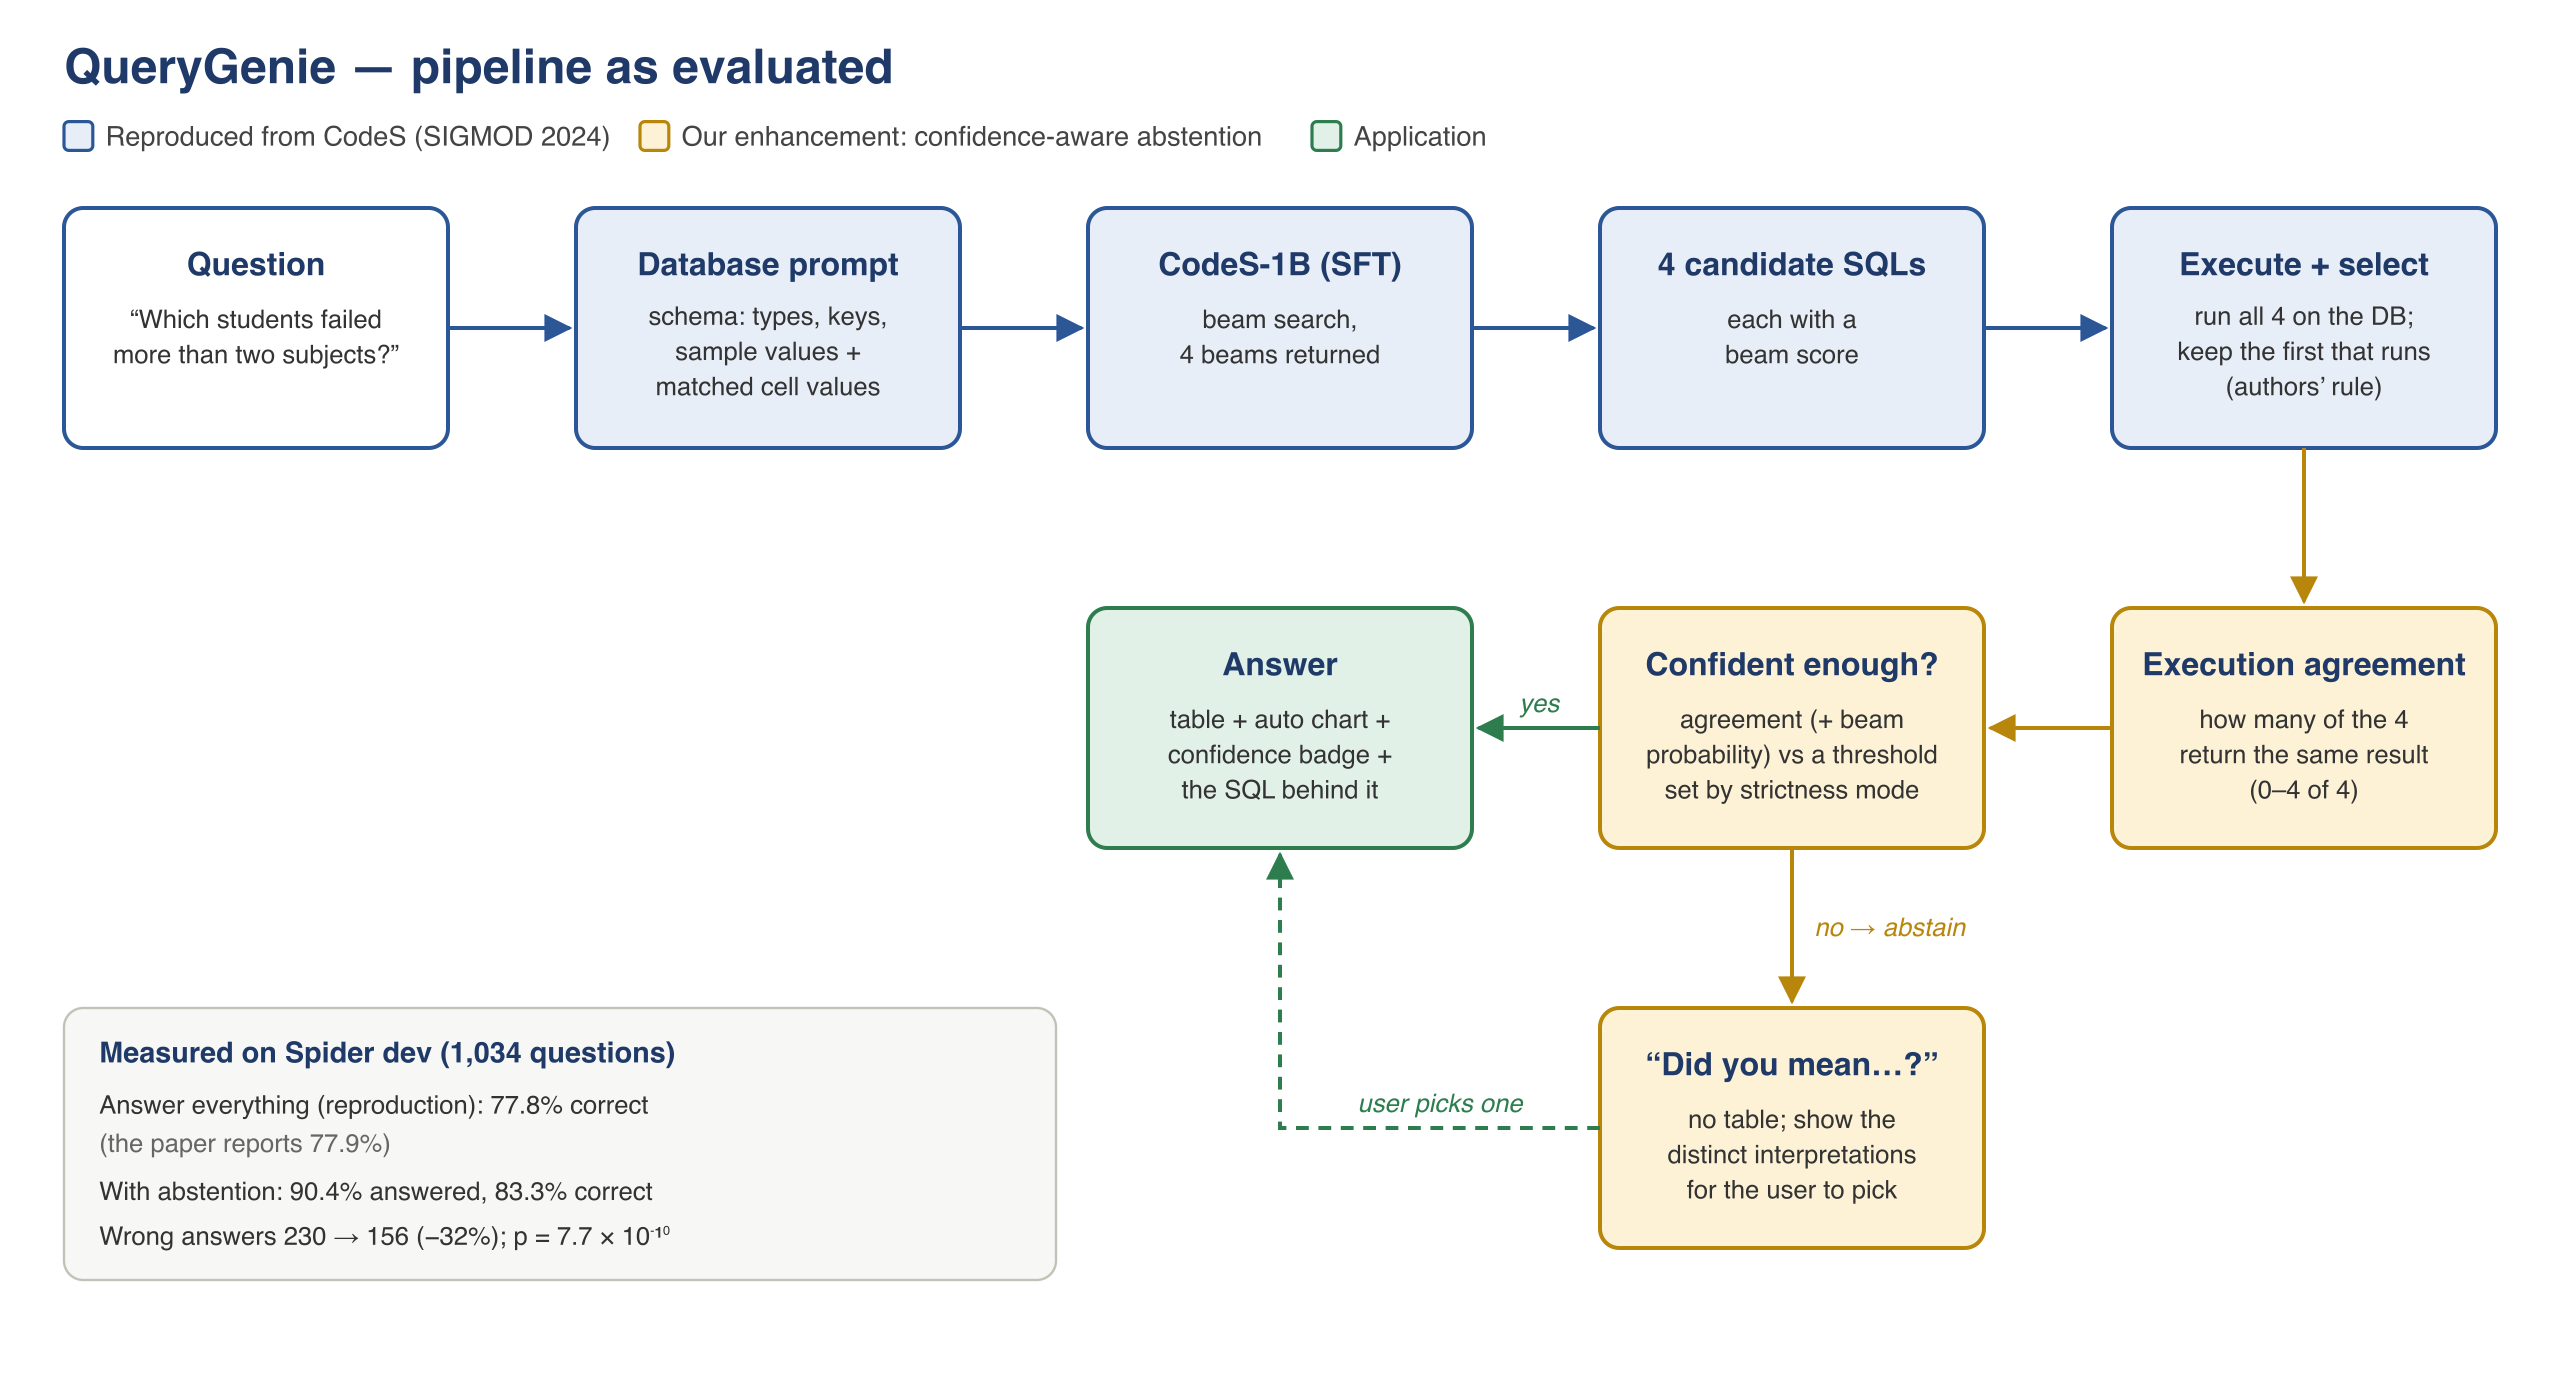
\includegraphics[width=\linewidth]{images/figures/final_pipeline.png}
	\caption{The pipeline as evaluated: reproduced CodeS components (blue), the enhancement (amber) and the application (green).}
	\label{fig:pipeline}
\end{figure}

\section{Reproduction methodology}

\subsection{The CodeS pipeline}

Given a question $Q$ and a database $D$, a text-to-SQL system produces a query $S$ whose result answers $Q$. CodeS builds the database prompt described in Chapter~3 --- schema sequence, column descriptions and the matched cell values --- and appends the question. A schema item classifier can prune the schema to its most relevant tables and columns. The model generates four candidates with beam search, and the first candidate that SQLite accepts is returned. Figure~\ref{fig:codes} summarises the pipeline as annotated from the paper.

\begin{figure}[!t]
	\centering
	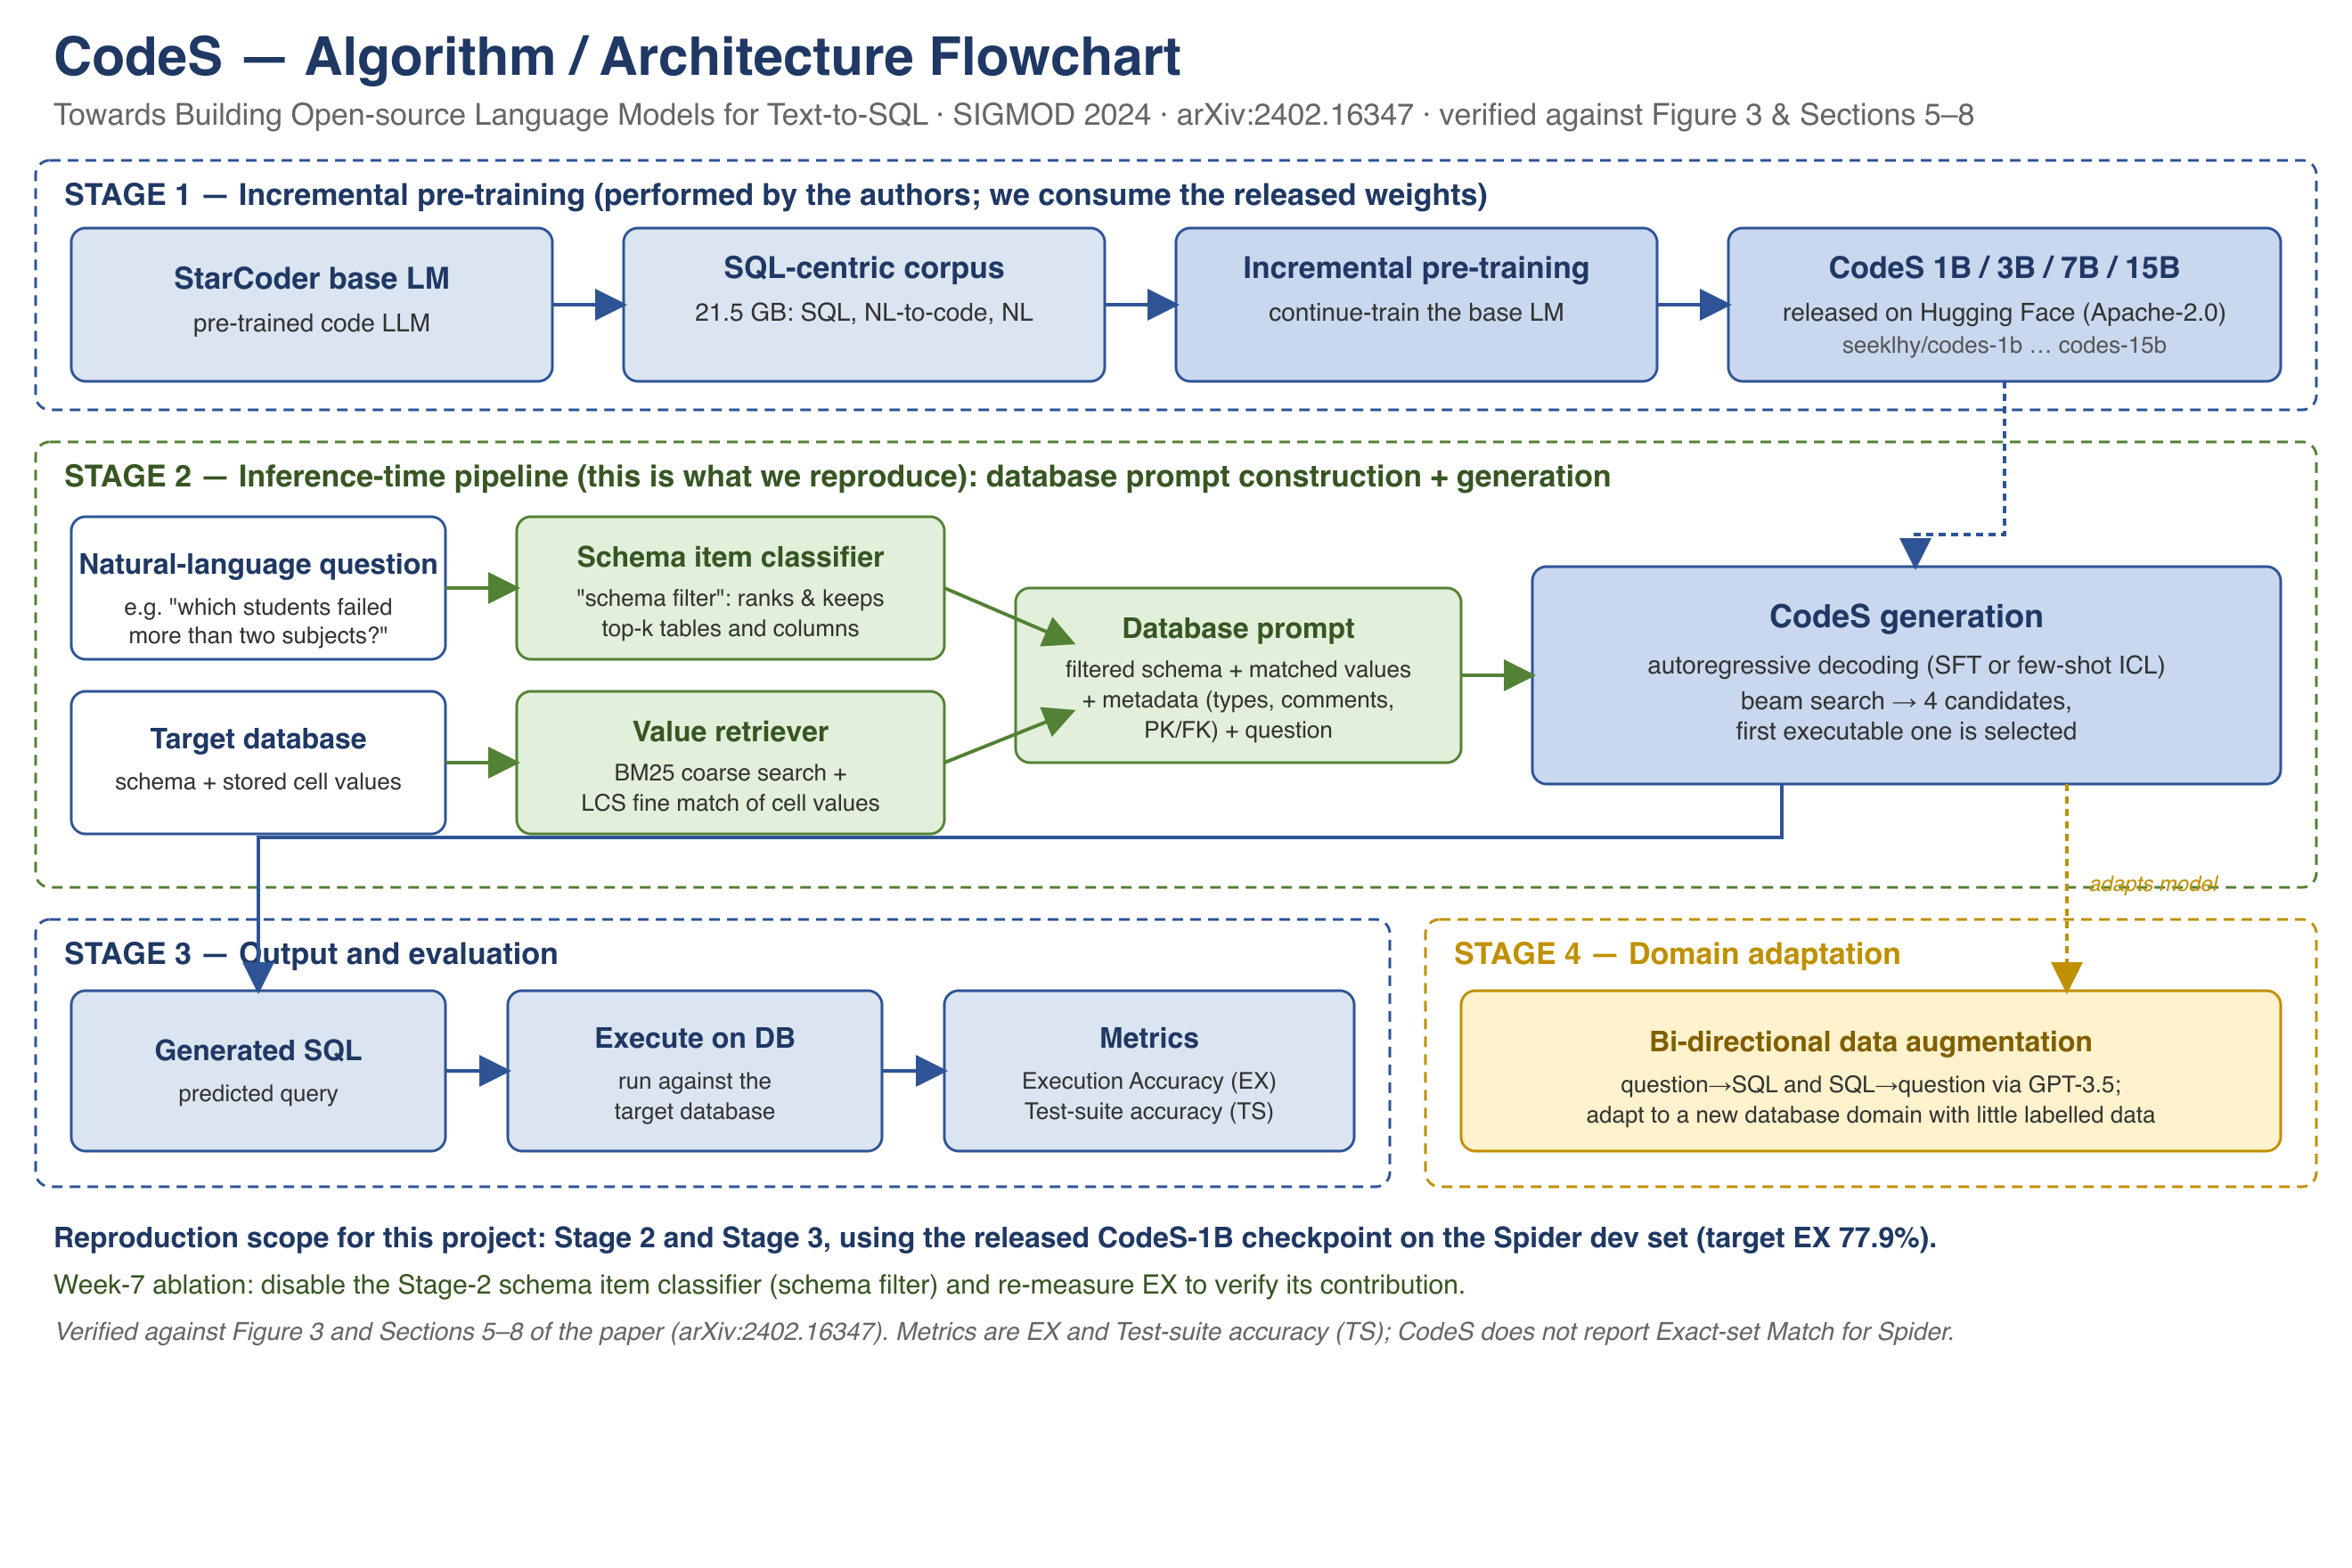
\includegraphics[width=0.92\linewidth]{images/figures/codes_architecture_flowchart.png}
	\caption{The CodeS pipeline, annotated from the paper (Week-3 deliverable).}
	\label{fig:codes}
\end{figure}

\subsection{Environment}

Table~\ref{tab:env} compares the authors' environment with ours. The reproduction first passed the department's Week-4 gate: the released model was loaded on a Colab T4 GPU, generated SQL and executed it against SQLite (run T1-001). The full evaluation followed.

\begin{table}[!t]
	\centering
	\caption{The authors' environment and ours.}
	\label{tab:env}
	\resizebox{\textwidth}{!}{%
	\begin{tabular}{|l|l|l|}
		\hline
		 & \textbf{Authors (official repository)} & \textbf{This project} \\ \hline
		GPU & 8 $\times$ NVIDIA A800, 80\,GB & NVIDIA Tesla T4, 16\,GB (Google Colab); Apple M4, 16\,GB for development \\ \hline
		Precision / batch & fp16, batch size 1 at inference & fp16, batch size 1 \\ \hline
		Python & 3.8.5 & Colab default (3.12.13 at the gate run) \\ \hline
		PyTorch & 1.13.1 & 2.11.0+cu128 \\ \hline
		transformers & 4.28.1 & 5.15.0 (gate run), 5.16.1 (reported runs) \\ \hline
		Dataset & Spider (Google Drive bundle) & Spider from Hugging Face (\path{xlangai/spider}, \path{HAL-9001/spider-databases}) \\ \hline
	\end{tabular}}
\end{table}

\subsection{The reproduced pipeline}

The evaluation harness (\path{research/colab_eval_tier2.py}) reproduces the authors' inference code, and the authors' database utilities are included unmodified (Apache-2.0):

\begin{itemize}
	\item \textbf{Prompt:} schema sequence, matched contents and question, with the beginning-of-sequence token and the authors' left-truncation, exactly as in their \path{prepare_text2sql_prefix_sequence}.
	\item \textbf{Value retriever:} the authors' fine matcher applied to every column's distinct values. The authors first narrow the candidates with a Lucene BM25 index; we scan all values instead (a documented deviation).
	\item \textbf{Decoding and selection:} beam search with four beams, all four returned and post-processed; the first candidate that passes SQLite's \texttt{EXPLAIN QUERY PLAN} is kept, otherwise the first beam --- the rule in the authors' \path{text2sql_zero_shot.py}.
	\item \textbf{Scoring:} the official Spider test-suite evaluator (\texttt{evaluation.py --etype exec}) \cite{zhong2020semantic}, which is what the authors call. Execution Accuracy (EX) counts a prediction as correct when it returns the same result as the gold query; the evaluator treats row order as significant only when the gold query sorts, tolerates reordered columns and ignores \texttt{DISTINCT} by default. Every prediction is saved so that any run can be re-scored.
\end{itemize}

\subsection{Audit of the evaluation harness}

After three runs gave 64.8\%, 71.7\% and 73.8\%, the harness was compared line by line with the authors' code (\path{load_sft_dataset.py}, \path{prepare_sft_datasets.py}, \path{build_contents_index.py}, \path{text2sql_zero_shot.py} and \path{db_utils.py}), and every effect was measured on the full development set. Prompt assembly, decoding, candidate selection and post-processing matched, and the vendored code was identical to the authors'. Four discrepancies were found and fixed:

\begin{enumerate}
	\item \textbf{Value-retriever bug.} The authors index every value as text, numbers included; our port kept only text values, so numbers in questions (``older than 20'') were never matched. This changed the prompt for 128 of the 1,034 questions (12.4\%).
	\item \textbf{Scoring metric.} Our early metric compared sorted rows as strings: it ignored row order and did not accept reordered columns. On the same predictions it gives 73.4\% where the official evaluator gives 77.8\%, so the earlier runs were not on the paper's scale.
	\item \textbf{Column descriptions.} The authors add human-readable column names from Spider's \path{tables.json}; 12 development-set columns are affected.
	\item \textbf{Saved predictions.} Earlier runs did not save their SQL and could not be re-scored.
\end{enumerate}

The official evaluator was checked by scoring the gold queries against themselves (1.000).

\subsection{Run logging and determinism}

Every run is logged with its seed (42), hardware, runtime and library versions in \path{results/reproduction_log.csv} and \path{results/Reproduction_Log.xlsx}, including runs that were later superseded. Beam search is deterministic: repeating a run returned exactly the same predictions (763 of 1,034 correct in T2-003 and its repeat; 759 of 1,034 on the simple metric in T2-005 and T2-006). Differences between runs therefore come from configuration changes, not chance.

\section{Reproducibility results}

\subsection{Run history}

Table~\ref{tab:runs} lists the runs on the development set. The reproduction reached its final figure in steps, and each step isolates a real effect: moving from a schema-only prompt to the authors' full database prompt raised the simple-metric score from 64.8\% to 71.7\%, the authors' candidate-selection rule raised it to 73.8\%, and the audit showed that most of the remaining gap was the scoring metric rather than the model.

\begin{table}[!t]
	\centering
	\caption{Runs on the Spider development set (1,034 questions). ``Simple'' is the early sorted-rows metric; only ``official'' matches the paper.}
	\label{tab:runs}
	\resizebox{\textwidth}{!}{%
	\begin{tabular}{|l|l|l|l|l|}
		\hline
		\textbf{Run} & \textbf{Configuration} & \textbf{Metric} & \textbf{EX} & \textbf{vs 77.9\%} \\ \hline
		T1-001 & Week-4 gate: codes-1b loads, generates and executes SQL (Colab T4) & liveness & passed & --- \\ \hline
		T2-001 & schema and foreign keys only; first beam; Apple M4 & simple & 64.8\% & not comparable \\ \hline
		T2-002 & full CodeS prompt; first beam; Colab T4 & simple & 71.7\% & not comparable \\ \hline
		T2-003 & + authors' candidate selection; Colab T4 (repeated identically) & simple & 73.8\% & not comparable \\ \hline
		T2-005 & audited harness (v2); Colab T4 & official & 77.8\% & $-0.1$ pts \\ \hline
		T2-006 & fresh re-run of T2-005 (Week-10 baseline) & official & 77.76\% (804/1,034) & $-0.14$ pts \\ \hline
	\end{tabular}}
\end{table}

\subsection{Headline comparison}

Scored with the paper's own evaluator, the reproduced CodeS-1B reaches \textbf{77.8\% Execution Accuracy against the reported 77.9\%}: a difference of 0.1 points, well inside the department's tolerance. The fresh Week-10 re-run gave the identical result (804 of 1,034 correct). 97.3\% of the predictions execute.

Test-suite accuracy (paper: 72.2\%) requires the distilled test-suite databases, which are distributed on Google Drive and were not obtained; our test-suite accuracy is \textbf{TBD}. The saved predictions of T2-006 can be scored for it without re-running the model.

\subsection{Ablation study}

Each component of the pipeline was disabled in turn and the full development set re-evaluated with the official evaluator (runs AB-103 to AB-106, Colab T4). Table~\ref{tab:ablation} and Figure~\ref{fig:ablation} give the results.

\begin{table}[!t]
	\centering
	\caption{Ablation study, official evaluator.}
	\label{tab:ablation}
	\begin{tabular}{|l|r|r|r|}
		\hline
		\textbf{Component removed} & \textbf{EX} & \textbf{Change} & \textbf{Executable} \\ \hline
		--- (full pipeline, T2-005) & 77.8\% & --- & 97.3\% \\ \hline
		Foreign-keys block & 76.9\% & $-0.9$ & 95.9\% \\ \hline
		Representative column values & 76.4\% & $-1.4$ & 98.1\% \\ \hline
		Candidate selection (first beam only) & 76.0\% & $-1.8$ & 94.1\% \\ \hline
		Value retriever (matched contents) & 75.9\% & $-1.9$ & 97.2\% \\ \hline
	\end{tabular}
\end{table}

\begin{figure}[!t]
	\centering
	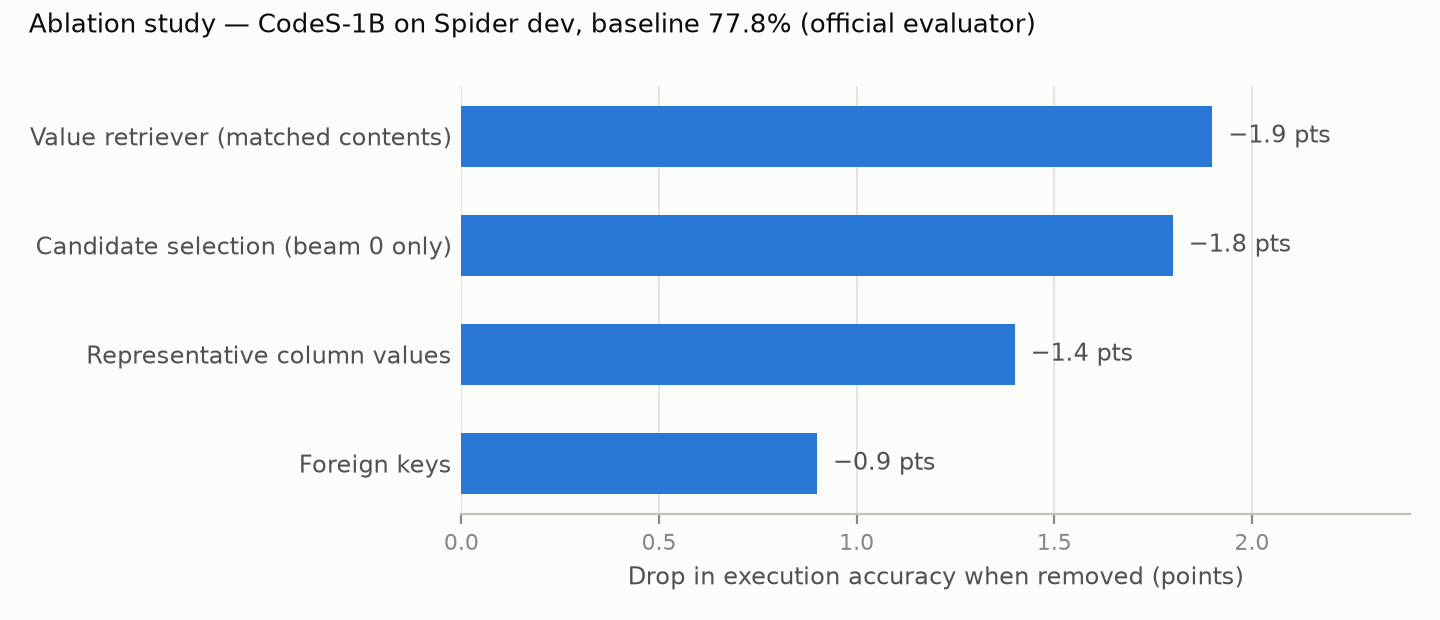
\includegraphics[width=0.8\linewidth]{images/figures/ablation_official.png}
	\caption{Drop in Execution Accuracy when each component is removed.}
	\label{fig:ablation}
\end{figure}

Every component contributes. The value retriever matters most, and the way it matters is telling: without it almost as many queries still execute (97.2\%) --- the model writes runnable SQL with the wrong literal values, so the answers are silently wrong. Candidate selection works differently: it is the ablation that reduces executability most (94.1\%), because it is what replaces a broken first beam with a working alternative. Without the foreign keys the model guesses join conditions, which also shows up as lower executability. These differences are 9 to 20 questions each and were not tested for significance individually.

\section{Enhancement: confidence-aware abstention}

\subsection{Choice and justification}

The department allows one enhancement, chosen from defined tiers and approved by the guide. The Week-1 abstract had named execution-guided self-correction, the strategy of DIN-SQL \cite{pourreza2023dinsql}. The reproduction showed that 97.3\% of predictions already execute, so repairing failed queries could recover at most 2.7 points and was unlikely to produce a significant gain. The ablation and the difficulty analysis of Chapter~3 showed instead that the dominant error is a query that runs but returns the wrong rows. We therefore proposed confidence-aware abstention (Tier 4, a novel combination), keeping self-correction and automatic charts as application features.

That expectation was later measured directly (\path{research/repair_eval.py}). Keeping the four candidates of run T2-006 fixed, every failed candidate --- 377 queries in 211 questions --- was sent back to CodeS-1B once with its database error. Only 61 of the repaired queries ran, and one answer became correct (none became wrong): Execution Accuracy moved from 77.76\% to 77.85\%, and the tested abstention setting from 90.43\% coverage at 83.32\% to 90.52\% at 83.23\%. CodeS was fine-tuned on question--SQL pairs and never learned to use error feedback, which DIN-SQL's self-correction relies on. Self-correction therefore remains an application feature, on by default and labelled as such, and is not part of the evaluated results.

\subsection{Method}

The pipeline already produces four beam candidates per question. All four are executed. The confidence of the returned answer is the share of candidates whose result equals it --- execution agreement, from 0 to 4 of 4, and zero when the returned query does not run --- with the beam probability of the returned candidate (the softmax of the four beam scores) used only to break ties. The idea combines self-consistency \cite{wang2022selfconsistency} with selective classification \cite{geifman2017selective}. When confidence is below a threshold the system abstains: it shows no table and offers the distinct results of the candidates as interpretations for the user to choose from. No retraining is involved. Algorithm~\ref{alg:abstain} states the procedure.

\begin{algorithm}[!t]
	\SetAlgoLined
	\KwIn{question $Q$, database $D$, threshold $\tau$}
	\KwOut{an answer, or the readings for the user to choose from}
	$P \leftarrow$ CodeS database prompt for $(Q, D)$\;
	$(s_1, \dots, s_4), (b_1, \dots, b_4) \leftarrow$ four beam candidates and their scores\;
	\For{$i \leftarrow 1$ \KwTo $4$}{
		$r_i \leftarrow$ result of executing $s_i$ on $D$ (read-only; empty if it fails)\;
	}
	$k \leftarrow$ first $i$ whose query passes \texttt{EXPLAIN QUERY PLAN}, else $1$\;
	$a \leftarrow \frac{1}{4}\,\lvert\{\, i : r_i = r_k \,\}\rvert$ if $s_k$ runs, else $0$\;
	$p \leftarrow e^{b_k} / \sum_j e^{b_j}$\;
	$c \leftarrow a + 0.01\,p$\;
	\eIf{$c \ge \tau$}{
		\Return result $r_k$ with confidence $a$\;
	}{
		\Return the distinct results among $r_1, \dots, r_4$ as readings\;
	}
	\caption{Confidence-aware abstention on top of CodeS}
	\label{alg:abstain}
\end{algorithm}

\subsection{Hypothesis and protocol}

The hypothesis and protocol were fixed before the results were seen.

\begin{itemize}
	\item \textbf{H1:} at the same coverage, accuracy on answered questions is higher with agreement-based abstention than with random abstention, and higher than the 77.8\% baseline. \textbf{H0:} no difference.
	\item \textbf{Protocol:} 10 random 50/50 splits of the development set. On the calibration half the threshold is set for at least 90\% coverage, then applied to the test half. The paired quantity is the accuracy on answered test questions minus the expected accuracy of random abstention at the same coverage, which is the test half's full-coverage accuracy. One-sided paired t-test and Wilcoxon signed-rank test, $\alpha = 0.05$.
	\item \textbf{Data:} one run (T2-006) recording, for every question, all four candidates with their beam scores, execution results and official correctness, checked to add up to the evaluator's total. The original and the enhanced systems are therefore compared on exactly the same predictions.
\end{itemize}

The threshold used by the application, $\tau = 0.2526$, is the median of the 10 calibration-half thresholds. In words: abstain when no candidate executes, or when only 1 of 4 candidates supports the answer and its beam probability is below about 0.26.

\subsection{Results}

Table~\ref{tab:enh} compares the original and enhanced systems on the same 1,034 questions, and Table~\ref{tab:sig} gives the significance tests.

\begin{table}[!t]
	\centering
	\caption{Original against enhanced on the same 1,034 questions.}
	\label{tab:enh}
	\resizebox{\textwidth}{!}{%
	\begin{tabular}{|l|r|r|r|}
		\hline
		\textbf{System} & \textbf{Answered} & \textbf{Accuracy on answered} & \textbf{Wrong answers} \\ \hline
		CodeS-1B, paper (Table 5) & 1,034 (100\%) & 77.9\% & --- \\ \hline
		Original --- CodeS-1B reproduced & 1,034 (100\%) & 77.76\% & 230 \\ \hline
		Enhanced --- tested setting & 935 (90.4\%) & 83.32\% & 156 \\ \hline
		Enhanced --- 3 of 4 agree & 649 (62.8\%) & 86.13\% & 90 \\ \hline
		Enhanced --- all 4 agree & 412 (39.8\%) & 88.35\% & 48 \\ \hline
	\end{tabular}}
\end{table}

\begin{table}[!t]
	\centering
	\caption{Significance tests over 10 calibration/test splits (mean coverage 90.5\%) and a 5,000-sample bootstrap over questions.}
	\label{tab:sig}
	\resizebox{\textwidth}{!}{%
	\begin{tabular}{|l|l|l|l|l|}
		\hline
		\textbf{Signal} & \textbf{Mean gain} & \textbf{Paired t-test (df 9)} & \textbf{Wilcoxon} & \textbf{Bootstrap 95\% CI} \\ \hline
		Execution agreement & $+5.46$ pts (SD 0.71) & $t = 24.44$, $p = 7.7 \times 10^{-10}$ & $W = 55$, $p = 9.8 \times 10^{-4}$ & $[+4.51, +6.71]$ \\ \hline
		Beam probability (comparison) & $+3.08$ pts (SD 0.90) & $t = 10.81$, $p = 9.3 \times 10^{-7}$ & $W = 55$, $p = 9.8 \times 10^{-4}$ & $[+1.97, +3.94]$ \\ \hline
	\end{tabular}}
\end{table}

H0 is rejected. All 10 splits showed a positive gain ($W = 55$ is the maximum, and $9.8 \times 10^{-4}$ the smallest p-value the Wilcoxon test can give with 10 pairs). Because the splits reuse the same questions, the questions themselves were also resampled 5,000 times; no resample showed a gain of zero or less. At the tested setting the system declines 99 questions, 74 of which it would have answered wrongly and 25 correctly: wrong answers fall by 32\% at the cost of withholding 3.1\% of the correct ones.

Figure~\ref{fig:coverage} shows the whole accuracy--coverage curve, and Table~\ref{tab:calib} shows that the signal is calibrated: accuracy rises steadily with agreement.

\begin{figure}[!t]
	\centering
	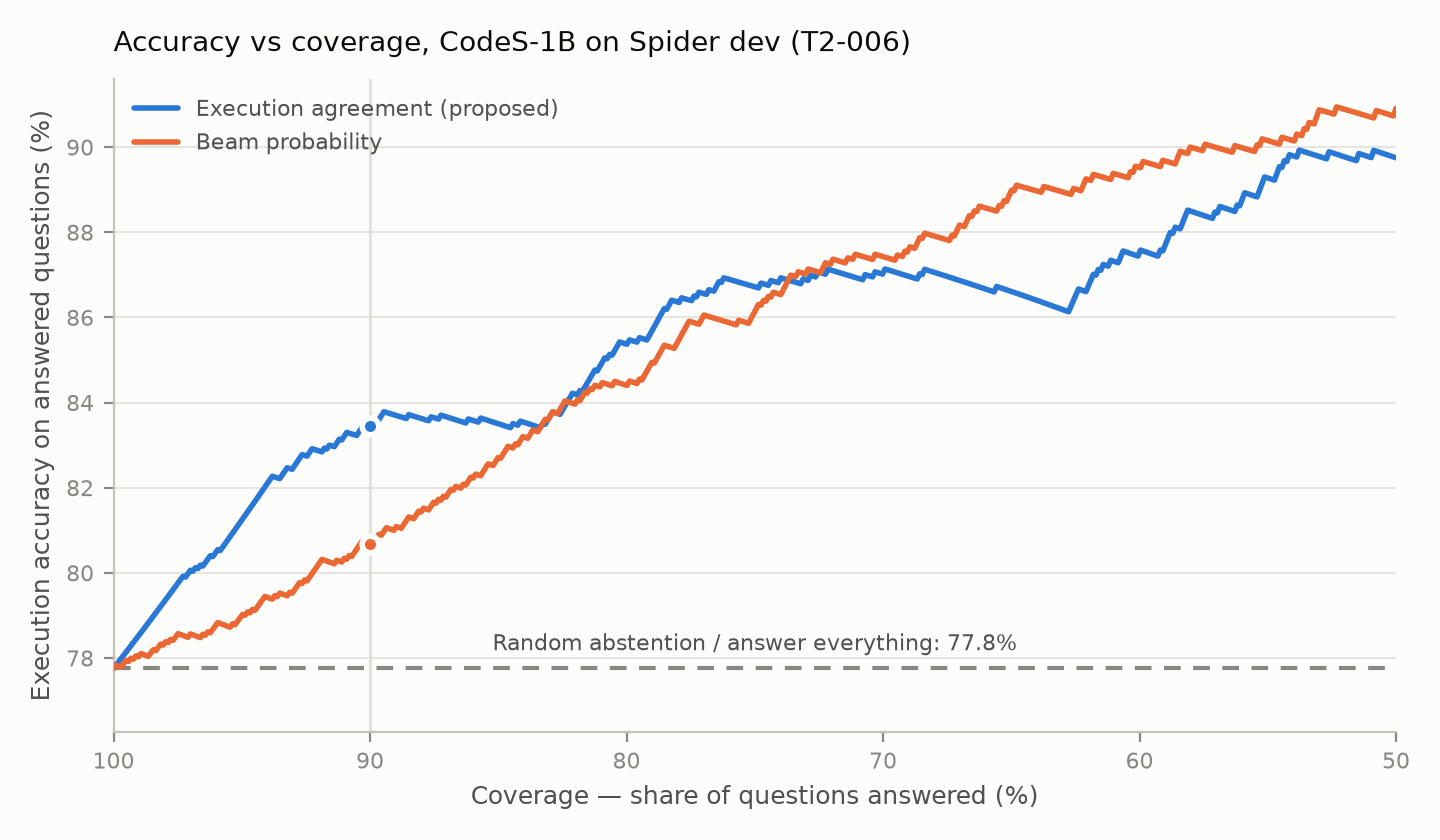
\includegraphics[width=0.8\linewidth]{images/figures/accuracy_coverage_T2-006.png}
	\caption{Accuracy on answered questions against coverage. The dashed line is the original system (and random abstention); dots mark 90\% coverage.}
	\label{fig:coverage}
\end{figure}

\begin{table}[!t]
	\centering
	\caption{Accuracy by the number of candidates agreeing with the answer.}
	\label{tab:calib}
	\begin{tabular}{|l|r|r|}
		\hline
		\textbf{Candidates agreeing with the answer} & \textbf{Questions} & \textbf{Accuracy} \\ \hline
		None (selected query does not run) & 28 & 0.0\% \\ \hline
		1 of 4 & 132 & 56.8\% \\ \hline
		2 of 4 & 225 & 75.6\% \\ \hline
		3 of 4 & 237 & 82.3\% \\ \hline
		4 of 4 & 412 & 88.3\% \\ \hline
	\end{tabular}
\end{table}

\subsection{Agreement for choosing, not only for abstaining?}

A natural question is whether agreement could also raise plain Execution Accuracy, by returning the answer most candidates agree on instead of the first one that executes. Table~\ref{tab:select} answers it from the same four-candidate record (\path{research/selection_analysis.py}; no model run). Majority vote is \emph{worse}: it changes the selection on 69 questions, 11 of which become correct and 32 wrong, so accuracy falls from 77.76\% to 75.73\%. When the candidates split, the first beam is right more often than the majority. Agreement is therefore a good signal for deciding \emph{whether} to trust an answer, which is how the enhancement uses it, but not for deciding \emph{which} answer to give.

\begin{table}[!t]
	\centering
	\caption{Choosing among the four candidates of run T2-006.}
	\label{tab:select}
	\begin{tabular}{|l|r|r|}
		\hline
		\textbf{Selection rule} & \textbf{Correct} & \textbf{EX} \\ \hline
		First candidate that executes (CodeS, reproduced) & 804 & 77.76\% \\ \hline
		Majority vote over the candidates' results & 783 & 75.73\% \\ \hline
		Upper bound: a correct candidate is among the four & 859 & 83.08\% \\ \hline
	\end{tabular}
\end{table}

The upper bound shows the room that remains: a correct query is among the four candidates for 83.1\% of questions, while the selection rule picks it for 77.8\%. Closing part of that gap would need a learned reranker, which is left as future work.

\subsection{Limits of the enhancement}

\begin{itemize}
	\item \textbf{Beam probability is the better signal when abstaining heavily.} Execution agreement is ahead from 100\% down to about 74\% coverage --- the region where a usable assistant operates and where the proposal set its operating point --- but below 74\% beam probability is ahead, and over the whole curve it has the lower area under the risk--coverage curve (0.091 against 0.103; random 0.222, perfect ranking 0.027).
	\item \textbf{Agreement is not proof.} 11.7\% of the answers on which all four candidates agree are still wrong; abstention reduces errors but does not remove them.
	\item \textbf{One model, one benchmark.} The threshold was calibrated on Spider with CodeS-1B; its behaviour with other models, and on real institutional databases, is not measured.
	\item \textbf{Statistical independence.} The 10 splits reuse the same questions, so their p-values are optimistic; the question-level bootstrap is the check that does not depend on this.
\end{itemize}

\section{The application}

The enhancement is delivered in QueryGenie, a desktop application for macOS and Windows, which meets the department's requirement for a full-stack deliverable rather than a notebook. On first start a setup assistant checks the computer and downloads the model (\path{seeklhy/codes-1b-spider}, about 4.5\,GB) and, optionally, the 20 Spider development databases. It then runs exactly the evaluated pipeline, locally.

\begin{itemize}
	\item \textbf{Chats.} Questions are asked in chats, one database at a time. Every answer shows how many of the four candidate queries agree (Figure~\ref{fig:app-answer}), the results table, an automatically chosen chart, the SQL behind the table (editable, and re-runnable read-only) and all four candidates.
	\item \textbf{Abstention.} When the candidates disagree beyond the chosen strictness setting, the application withholds the table and shows the distinct readings for the user to choose from (Figure~\ref{fig:app-notsure}). The four strictness settings display their measured coverage and accuracy from Table~\ref{tab:enh}.
	\item \textbf{Schema map.} The whole database is drawn as a tree of tables, columns, keys and links; tapping a table or column offers questions about it (Figure~\ref{fig:app-map}).
	\item \textbf{Databases.} Besides the sample and Spider databases, users can open their own SQLite files or connect to PostgreSQL and MySQL servers. Every query is checked to be a single read-only statement and runs inside a read-only transaction with a timeout and a row limit. The model writes SQLite-style SQL, which is translated to the server's dialect: on the Spider databases loaded into PostgreSQL, translated queries return the same answer as on SQLite for 94.4\% of gold queries and 93.7\% of the model's predictions. Accuracy and confidence were calibrated on SQLite only.
	\item \textbf{Other models.} The evaluated CodeS-1B model is the default. The user can also choose the earlier prototype's CodeS variants, any model run by Ollama, an OpenAI-compatible server, or cloud services (Figure~\ref{fig:app-picker}). They receive the same four-candidate confidence check, but their accuracy was not measured, and the application labels their confidence as not calibrated. Cloud services receive the schema, a few example values and the question, never result rows, and only after the user confirms.
\end{itemize}

By default everything runs on the user's computer on open weights, so no schema or data leaves the machine.

\begin{figure}[!t]
	\centering
	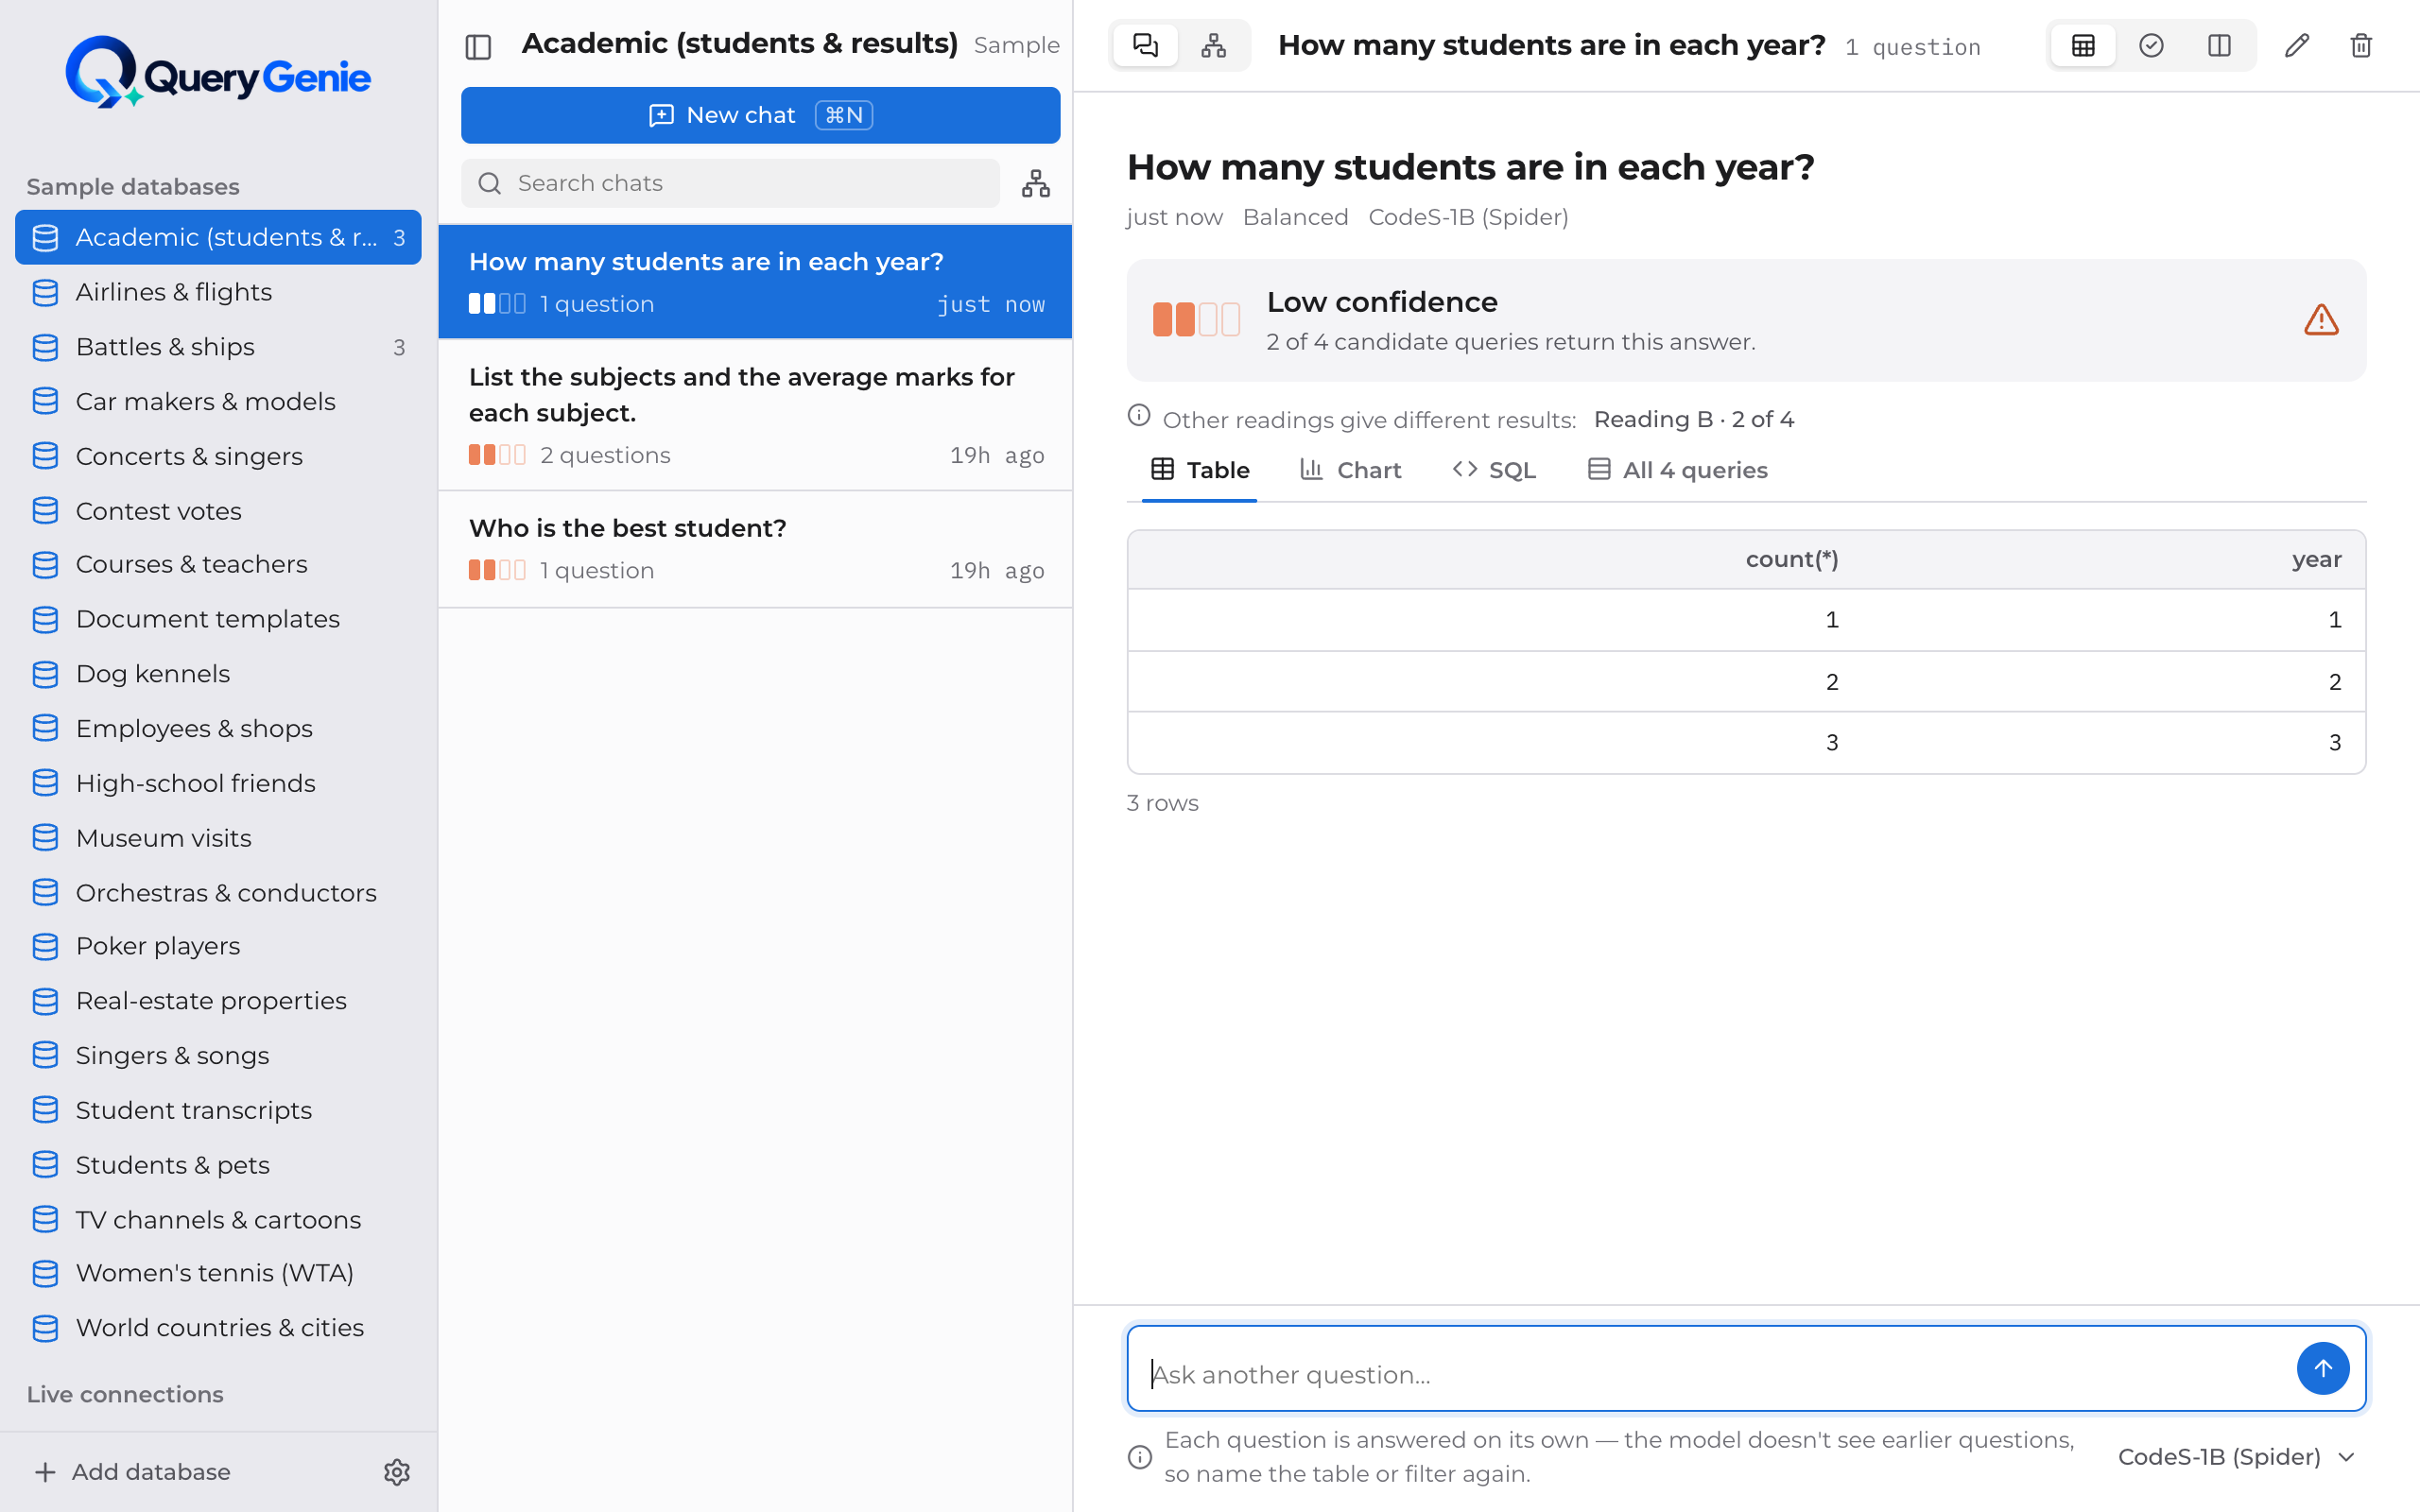
\includegraphics[width=\linewidth]{images/figures/app_answer.png}
	\caption{An answer with its confidence: two of the four candidate queries agree, so the answer is shown as low confidence, with the other reading offered.}
	\label{fig:app-answer}
\end{figure}

\begin{figure}[!t]
	\centering
	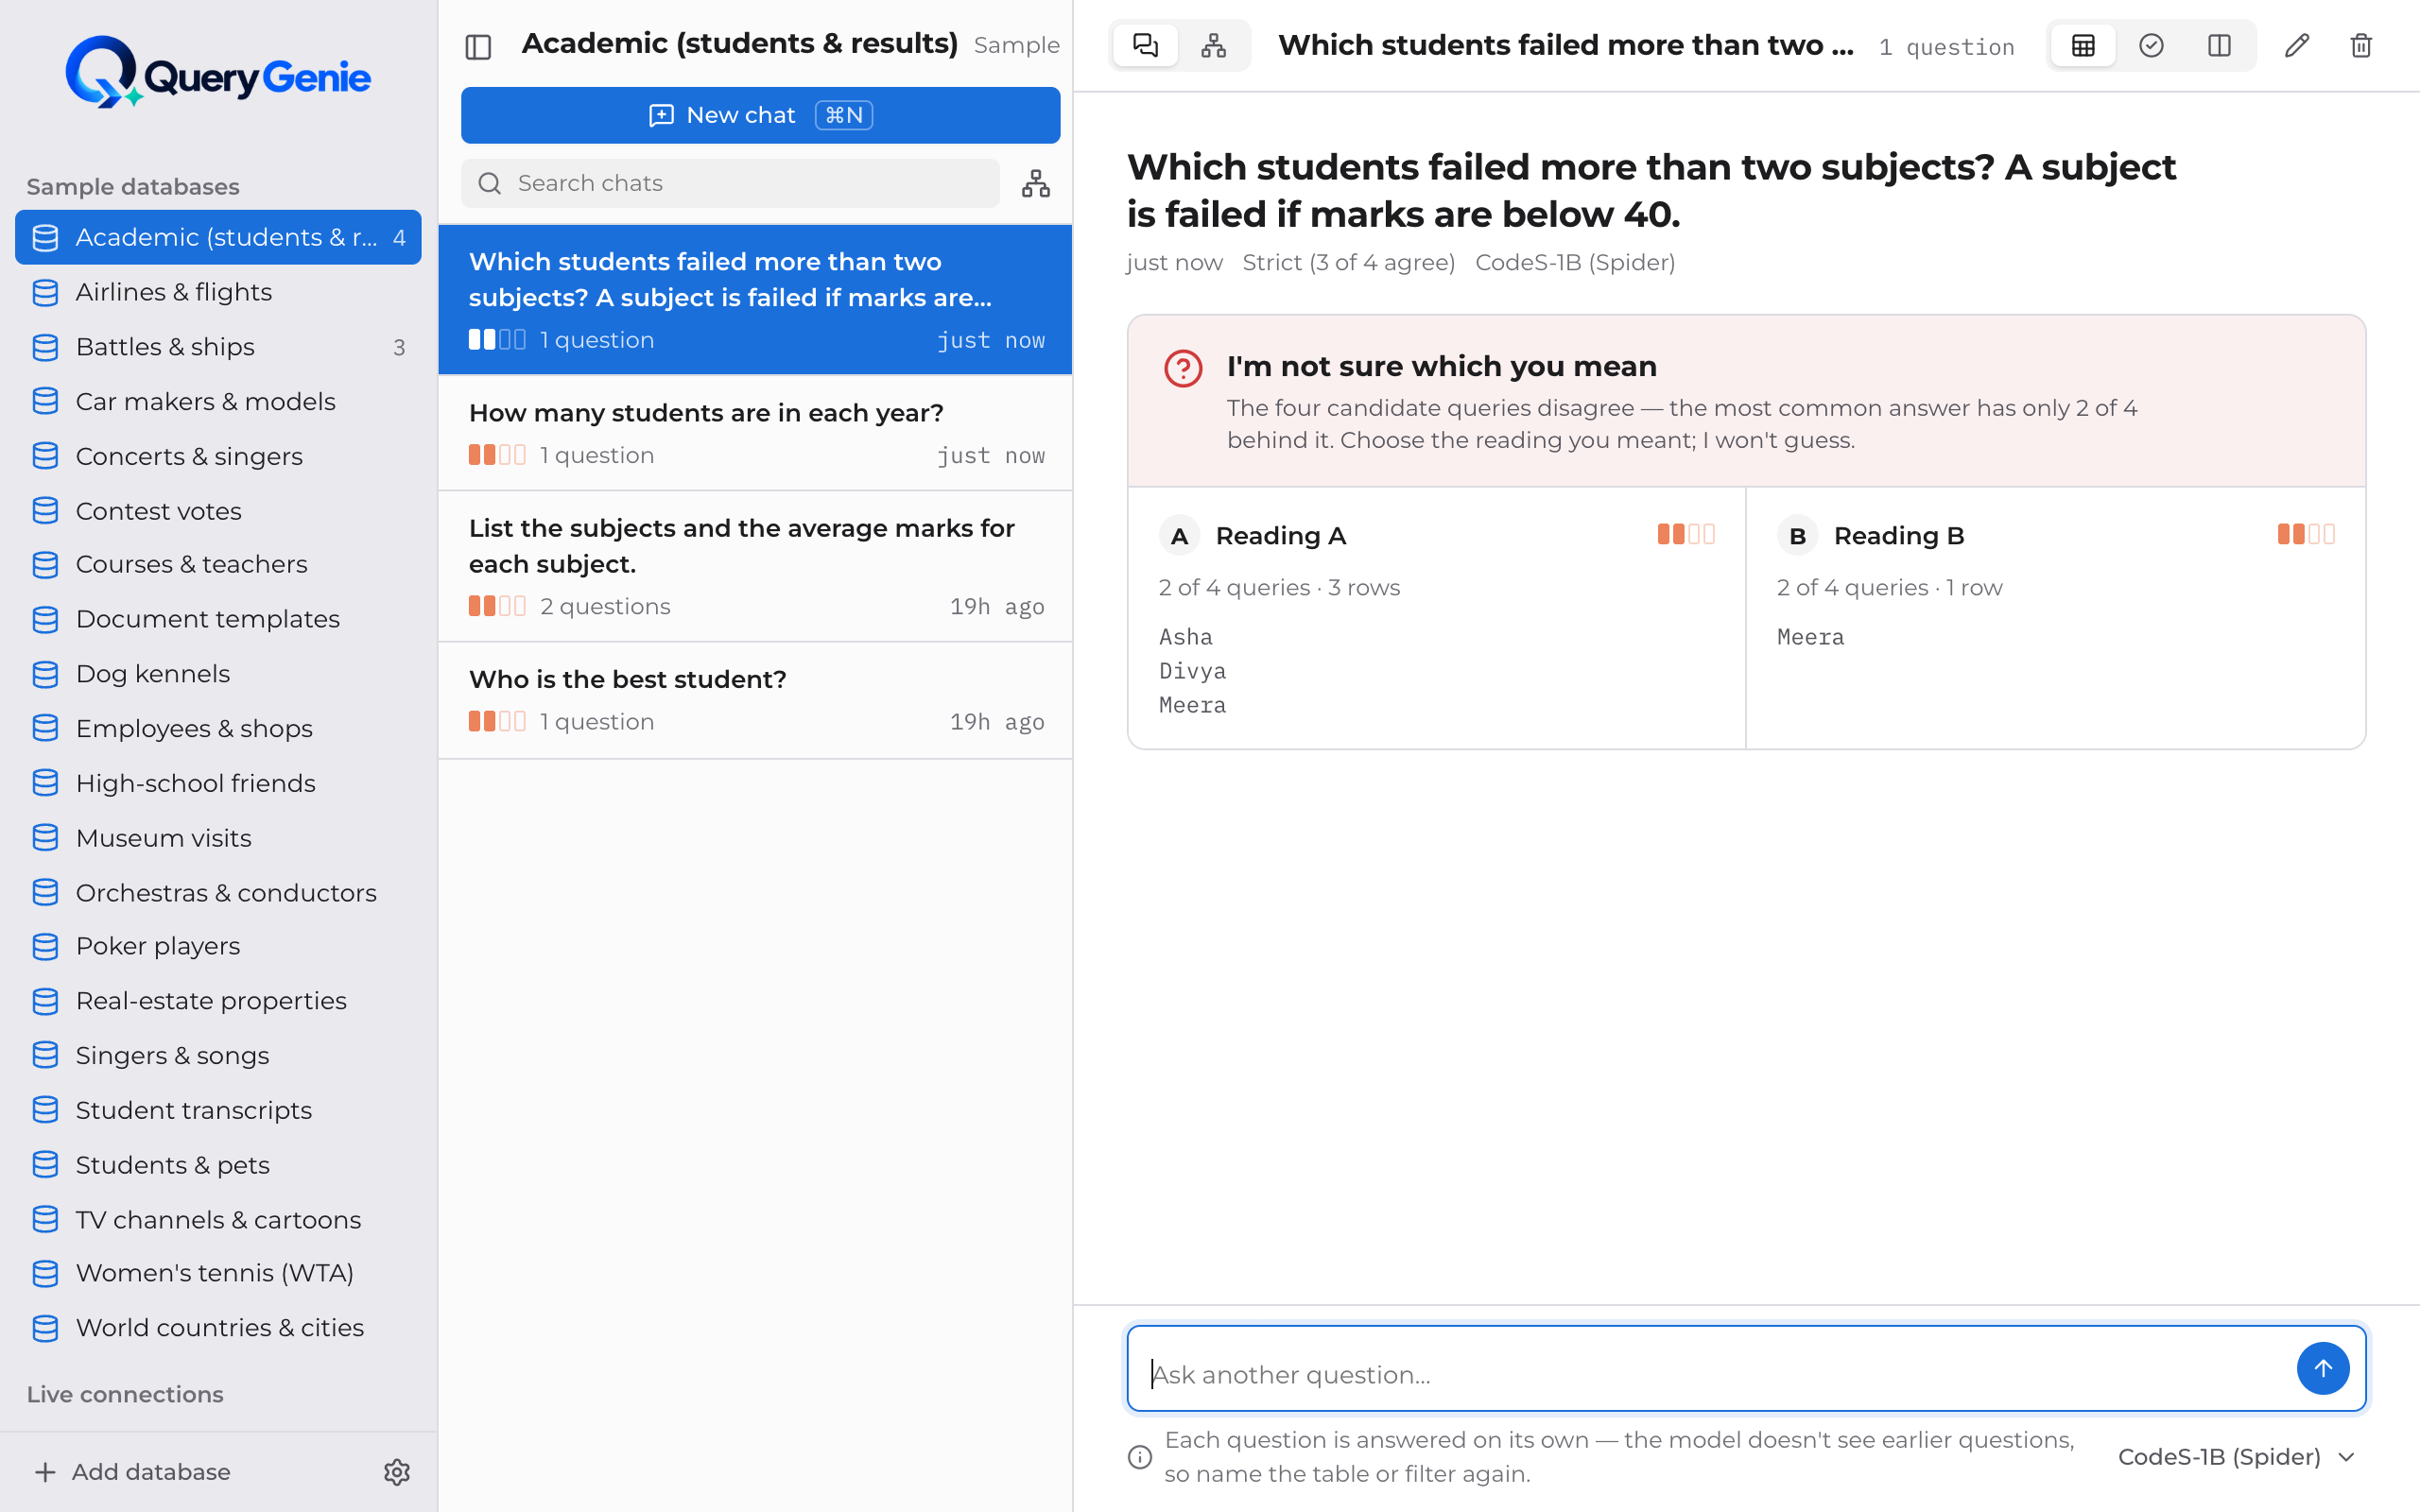
\includegraphics[width=\linewidth]{images/figures/app_not_sure.png}
	\caption{Abstention under the strict setting: the candidates split two against two on the flagship question, so the application asks which reading was meant instead of guessing.}
	\label{fig:app-notsure}
\end{figure}

\begin{figure}[!t]
	\centering
	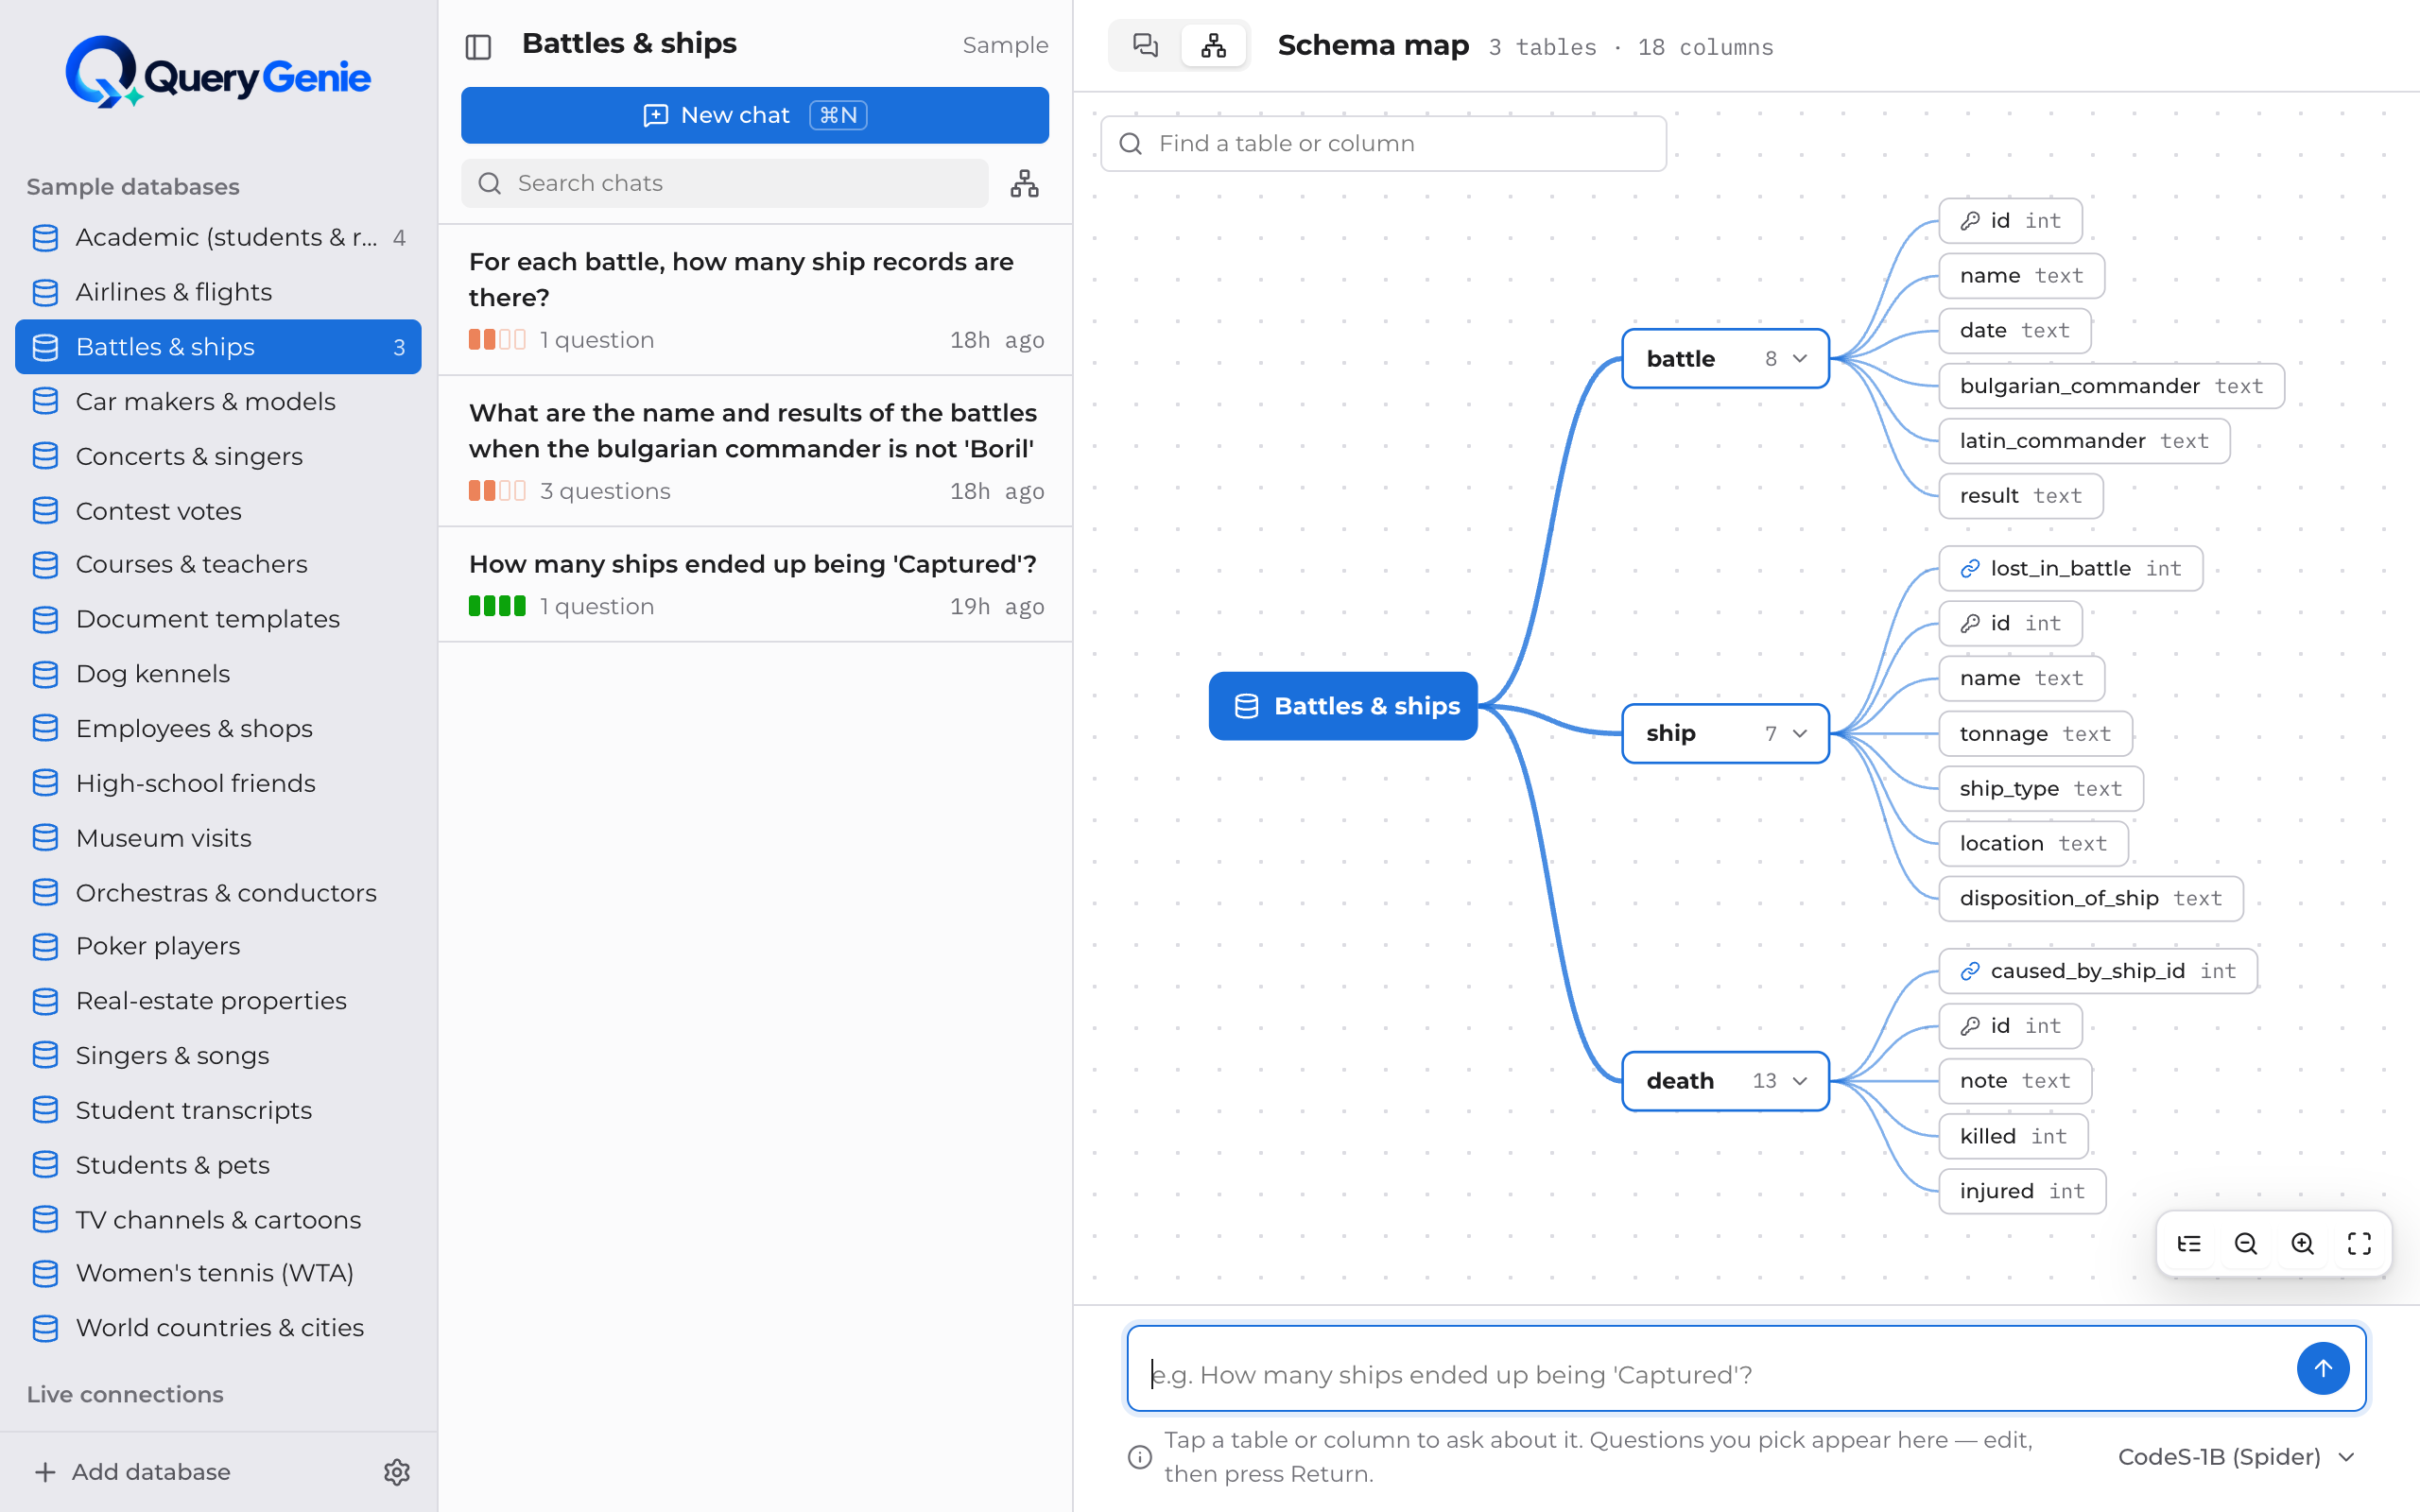
\includegraphics[width=\linewidth]{images/figures/app_schema_map.png}
	\caption{The schema map: tables, columns, primary keys and foreign keys of a Spider database.}
	\label{fig:app-map}
\end{figure}

\begin{figure}[!t]
	\centering
	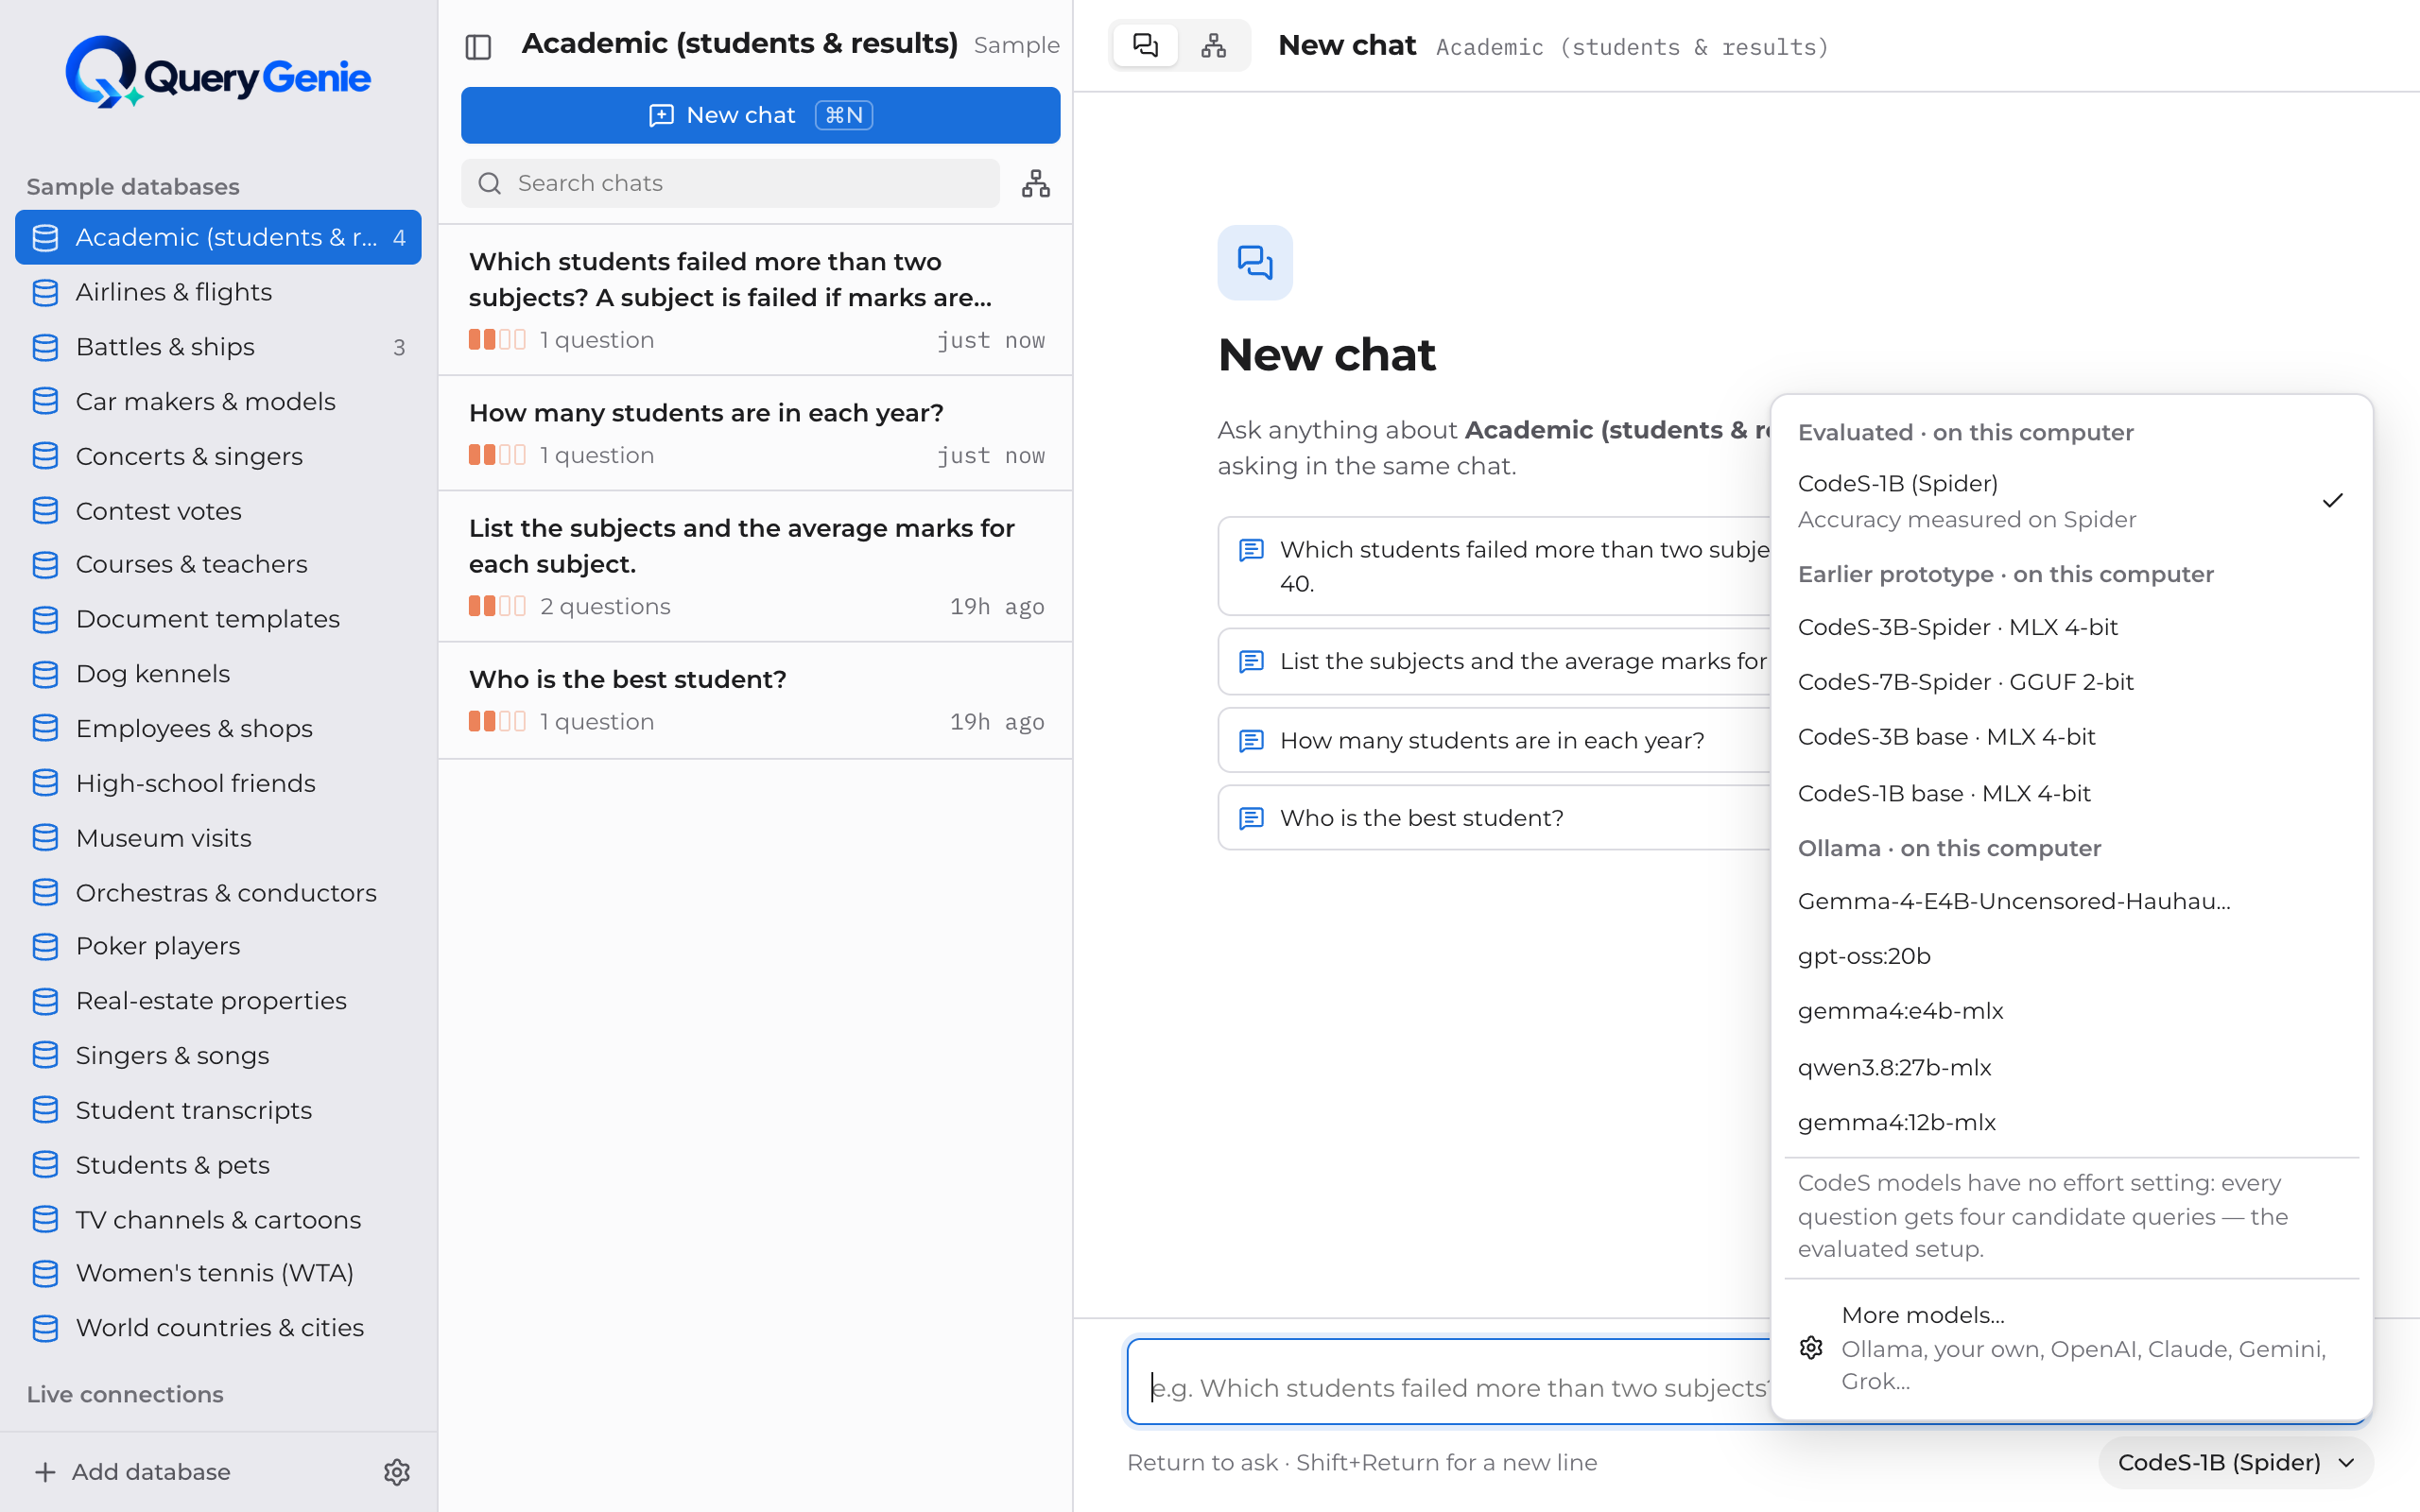
\includegraphics[width=\linewidth]{images/figures/app_model_picker.png}
	\caption{The model picker below the question box: the evaluated model, the earlier prototype's models and local Ollama models.}
	\label{fig:app-picker}
\end{figure}

A qualitative check on the bundled academic database shows both sides of the behaviour (illustrative, not a metric). With CodeS-1B the flagship question ``Which students failed more than two subjects?'' gets a wrong first answer, but the candidates split two against two, the answer is marked low confidence, the correct reading is offered as an alternative, and the strict setting abstains (Figure~\ref{fig:app-notsure}). A system that says when it is unsure is only as useful as that signal is honest, which is why the application shows its measured operating points rather than a single headline number.

\section{Differences from the authors' setup}

The reproduced accuracy is within 0.1 points of the paper, so the remaining deviations appear to have little effect on this benchmark. They are recorded in Table~\ref{tab:dev} for completeness.

\begin{table}[!t]
	\centering
	\caption{Remaining deviations from the authors' setup.}
	\label{tab:dev}
	\resizebox{\textwidth}{!}{%
	\begin{tabular}{|l|l|l|}
		\hline
		\textbf{Deviation} & \textbf{Cause} & \textbf{Observed or expected effect} \\ \hline
		Newer PyTorch and transformers & The pinned stack does not build on current Python & The authors note newer versions shift inference slightly; no measurable gap remains \\ \hline
		Distinct-value scan instead of Lucene BM25 & Avoids the Java / pyserini dependency & Superset of the authors' candidates; matched values may differ in number and order \\ \hline
		Schema item classifier not applied & Checkpoints on rate-limited Google Drive & Full schema passed; Spider databases are small \\ \hline
		Tesla T4 instead of A800 & Available hardware & Same precision (fp16) and batch size (1) as the authors' inference \\ \hline
		EX only; test-suite accuracy TBD & Test-suite databases not obtained & Test-suite accuracy (paper: 72.2\%) not yet reported \\ \hline
		Repository uses DeepSpeed ZeRO-2; paper states ZeRO-3 & Found while annotating the paper & Affects pre-training only, which was not reproduced \\ \hline
	\end{tabular}}
\end{table}

The largest lesson of the reproduction is about measurement rather than modelling. For a month our numbers sat 4 to 13 points below the paper, and the gap was blamed in turn on the prompt, the value retriever and the schema filter. The audit showed that about 4.4 points of it were our own scoring. Reproducing a result means reproducing the evaluation, not only the model.

\section{Source code and how to run it}

All code, results and documents are in the project repository on GitHub, \url{https://github.com/jayakanthh/QueryGenie}, with the supervisor added as a collaborator. The code is released under the Apache 2.0 licence. The repository is organised as follows:

\begin{itemize}
	\item \path{querygenie/} --- the evaluated core: the CodeS pipeline, the model wrapper, the abstention logic, the database catalogue and the connectors; the authors' utilities are included unmodified.
	\item \path{desktop/} --- the desktop application (native window, interface, first-run setup, packaging).
	\item \path{research/} --- the Colab evaluation harness, the abstention analysis, the dataset analysis of Chapter~3 and the notebooks.
	\item \path{results/} --- the run log, the harness audit, the ablation, abstention and comparison results, the figures, and the four-candidate record of run T2-006.
	\item \path{legacy/} --- the earlier web prototype, kept for the record; \path{tests/} --- model-free tests.
\end{itemize}

\textbf{Reproduce the results (GPU, about one hour).} Open \path{research/notebooks/02_tier2_colab_eval.ipynb} in Google Colab with a T4 runtime and run the Week-10 cell. It downloads Spider and the model from Hugging Face, evaluates all 1,034 questions with the official evaluator, and saves the predictions and the four-candidate record.

\textbf{Reproduce the enhancement analysis (CPU, seconds).}
\begin{lstlisting}[language=bash, caption={Significance tests, operating points and the accuracy--coverage figure}]
python research/abstention.py results/dump_T2-006.jsonl
\end{lstlisting}

\textbf{Run the application.}
\begin{lstlisting}[language=bash, caption=Running QueryGenie from source]
python3 -m venv .venv && source .venv/bin/activate
pip install -r requirements.txt
python desktop/main.py
\end{lstlisting}

\textbf{Tests (no model needed).} \texttt{python -m pytest tests/ -q}.


\chapter{Conclusion and Future Scope of work}
\section{Conclusion}

This project reproduced CodeS \cite{li2024codes}, an open-source text-to-SQL model, and extended it so that it says when it is unsure.

The fine-tuned CodeS-1B model was reproduced to within 0.1 points of its published Spider result: 77.8\% Execution Accuracy against 77.9\%, scored with the official evaluator, on hardware far smaller than the authors'. Getting there required an audit of our own evaluation harness, which traced most of an apparent 4--13 point gap to the scoring metric and a value-retriever bug rather than to the model. An ablation study showed that every part of the CodeS database prompt contributes 0.9 to 1.9 points, with the value retriever mattering most.

On top of the reproduced model, confidence-aware abstention uses the agreement between the four candidate queries CodeS already produces. At the pre-registered operating point it answers 90.4\% of questions and is correct on 83.3\% of them, against 77.8\% when answering everything, and it removes about a third of the wrong answers (230 to 156). The improvement is significant under a paired t-test, a Wilcoxon signed-rank test and a question-level bootstrap. Accuracy rises steadily with the number of agreeing candidates, from 56.8\% when only one agrees to 88.3\% when all four do, so the signal is calibrated.

The system is delivered as QueryGenie, a desktop application that runs the evaluated pipeline locally, shows how sure it is on every answer, and asks which reading the user meant when its candidates disagree.

\section{Future scope of work}

\begin{enumerate}
	\item \textbf{Test-suite accuracy.} Score the saved predictions of run T2-006 on the distilled test-suite databases, to report the stricter metric the paper also gives (72.2\%).
	\item \textbf{Larger models.} Evaluate CodeS-3B (paper: 83.4\%) and calibrate the abstention threshold for it rather than reusing the 1B threshold.
	\item \textbf{A learned reranker.} A correct query is among the four candidates for 83.1\% of questions but is selected for 77.8\%; a reranker trained to choose among them could raise plain Execution Accuracy, which majority voting does not (it lowers it to 75.7\%).
	\item \textbf{A combined signal.} Combine execution agreement and beam probability, which lead at different coverages, into one confidence score tuned only on calibration data.
	\item \textbf{The benchmark-to-reality gap.} Measure accuracy and abstention on a real institutional schema, where names, values and questions are messier than in Spider.
	\item \textbf{More databases.} Extend the connectors to further SQL engines and data warehouses, and to document stores through a local SQL snapshot, measuring translation accuracy for each as was done for PostgreSQL.
	\item \textbf{Other models.} Measure the accuracy and calibration of the other models the application can use, so that their confidence can be presented with the same evidence as CodeS-1B's.
\end{enumerate}
 

\clearpage

\newpage\phantomsection%
\addcontentsline{toc}{chapter}{\indexname}                   % add Index to TOC
\printindex


\onehalfspacing
\addcontentsline{toc}{chapter}{Bibliography}


\bibliographystyle{IEEEtran}
\bibliography{references}

\clearpage
\addcontentsline{toc}{chapter}{Biography}
\textbf{N V V S S Jayakanth Kamisetti} (2320090050) is a B.Tech student in Computer Science \& Information Technology at Koneru Lakshmaiah Education Foundation, Bowrampet, Hyderabad.

\textbf{Boddupally Narendar} (2320090009) is a B.Tech student in Computer Science \& Information Technology at Koneru Lakshmaiah Education Foundation, Bowrampet, Hyderabad.

\textbf{M Praneeth Reddy} (2320090018) is a B.Tech student in Computer Science \& Information Technology at Koneru Lakshmaiah Education Foundation, Bowrampet, Hyderabad.



%\newpage
%\clearpage
%\thispagestyle{plain}
%\begin{figure}
%	\centering
%	\includegraphics[width=\textwidth]{phdComic.pdf}
%\end{figure}
%\appendix
%\addcontentsline{toc}{chapter}{Appendix:}



% that's all folks
\end{document}
